%-------------------------------------------------------------------------------
% Document & Package declarations
%-------------------------------------------------------------------------------

\documentclass[a4paper, 10pt, conference]{ieeeconf}
\usepackage{graphicx}
\usepackage[colorlinks=true, allcolors=black]{hyperref}
\usepackage{tabularx}

%% Language and font encodings
\usepackage[english]{babel}
\usepackage[utf8x]{inputenc}
\usepackage[T1]{fontenc}

%% Useful packages
\usepackage{amsmath}
\usepackage{graphicx}
\usepackage[colorinlistoftodos]{todonotes}
% IEEEConf includes settings for caption/subcaption already!
% \usepackage[font=footnotesize,labelfont=bf]{caption}
\usepackage[font=footnotesize,labelfont=bf]{subcaption}
\usepackage{gensymb}

%% Packages for displaying source code
\usepackage{listings}
% \usepackage[framed,numbered,autolinebreaks,useliterate]{mcode}

\usepackage{float}
\usepackage{longtable}

%% Packages for displaying source code
\usepackage[numbered,framed]{matlab-prettifier}
\usepackage{color}

%%*************************************************************************
%% Legal Notice:
%% This code is offered as-is without any warranty either expressed or
%% implied; without even the implied warranty of MERCHANTABILITY or
%% FITNESS FOR A PARTICULAR PURPOSE!
%% User assumes all risk.
%% In no event shall IEEE or any contributor to this code be liable for
%% any damages or losses, including, but not limited to, incidental,
%% consequential, or any other damages, resulting from the use or misuse
%% of any information contained here.
%%
%% All comments are the opinions of their respective authors and are not
%% necessarily endorsed by the IEEE.
%%
%% This work is distributed under the LaTeX Project Public License (LPPL)
%% ( http://www.latex-project.org/ ) version 1.3, and may be freely used,
%% distributed and modified. A copy of the LPPL, version 1.3, is included
%% in the base LaTeX documentation of all distributions of LaTeX released
%% 2003/12/01 or later.
%% Retain all contribution notices and credits.
%% ** Modified files should be clearly indicated as such, including  **
%% ** renaming them and changing author support contact information. **
%%
%% File list of work: IEEEtran.cls, IEEEtran_HOWTO.pdf, bare_adv.tex,
%%                    bare_conf.tex, bare_jrnl.tex, bare_jrnl_compsoc.tex,
%%                    bare_jrnl_transmag.tex
%%*************************************************************************

%-------------------------------------------------------------------------------
% Document Configuration
%-------------------------------------------------------------------------------

\begin{document}
\title{Machine Learning for Computer Vision - Image Matching}
\author{Michael~Hart (00818445) and
        Meng~Kiang~Seah (00699092)
\\
        Department of Electrical and Electronic Engineering,
        Imperial College London,
        SW7 2AZ
\\
        E-mail: \{mh1613, mks211\}@imperial.ac.uk}
\date{\today}

%-------------------------------------------------------------------------------
% Plan on what to write
%-------------------------------------------------------------------------------

% See coursework instructions at:
% https://bb.imperial.ac.uk/bbcswebdav/pid-1034737-dt-content-rid-3589968_1/courses/DSS-EE4_62-16_17/MLCVCoursework2.pdf

%-------------------------------------------------------------------------------
% Information Banner
%-------------------------------------------------------------------------------

\maketitle

%-------------------------------------------------------------------------------
% Abstract
%-------------------------------------------------------------------------------

% \begin{abstract}
% Lorem ipsum dolor sit amet, consectetur adipiscing elit. Phasellus gravida viverra sollicitudin. Nulla ornare enim in ante auctor rhoncus a vel nulla. Nulla condimentum massa rhoncus, sodales arcu a, euismod nulla. Proin viverra mauris at massa molestie, a ultricies tortor fermentum. Duis consectetur, ante a tincidunt euismod, augue diam varius dolor, ut vestibulum orci est sit amet mi.
%
% \end{abstract}

%-------------------------------------------------------------------------------
% Introduction
%-------------------------------------------------------------------------------
\section{Introduction}
% Paper considers what?
% What data is used?
% What are the methods discussed? Short explanations

This paper uses computer vision methods to analyse and transform images, investigating the success of a few methods to accomplish this task. All implementations are written in MATLAB, and relevant files are given in the Appendix, referred to throughout the text using \texttt{typewriter} font. The images used are from the Tsukuba image set \cite{tsukuba}, the boat image set \cite{boat}, or from ``kitchen'' images taken by the authors. This latter set includes an FD image set, where the images are displaced by 0cm (FD1), 20cm (FD2), and 40cm (FD3); and an HG image set, where each image is tilted by 20\degree, and zoomed by factor 1.5, such that HG1 has focal length 24mm, HG2 has 36mm, and HG3 has 56mm.

\section{Question 1 - Matching}
\subsection{Manual Point Matching}

% Maybe a bit overkill considering our page limit, butt fuck it
In this method, five pairs of points are selected by the user (\texttt{q1\_manual.m}). An example of two images with the selected data points is shown in Figure \ref{fig:manual}.

\begin{figure}[!ht]
  \captionsetup[subfigure]{position=b}
  \centering
    \begin{subfigure}{0.45\linewidth}
      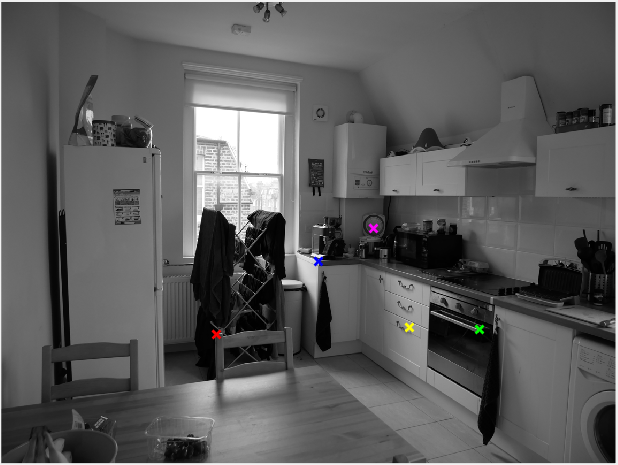
\includegraphics[width=\textwidth]{pic/manualA}
      \caption{Image HG1}
      \label{fig:manualA}
    \end{subfigure}
    ~
    \begin{subfigure}{0.45\linewidth}
      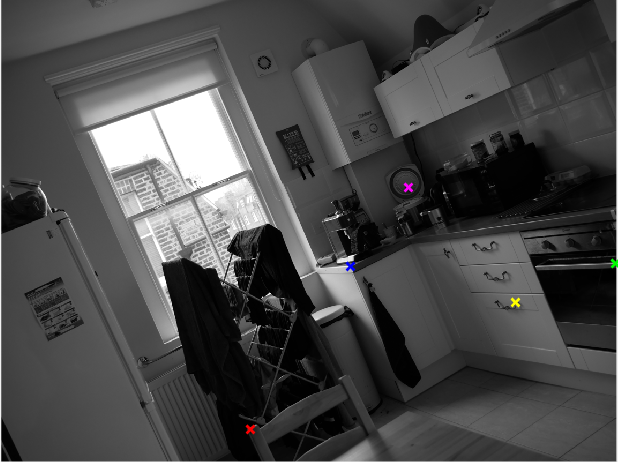
\includegraphics[width=\textwidth]{pic/manualB}
      \caption{Image HG2}
      \label{fig:manualB}
    \end{subfigure}

	\caption{Example of manually selected data points on images}
    \vspace{-0.75cm}
  \label{fig:manual}
\end{figure}

\subsection{Automatic Point Matching }
\subsubsection{Interest Point Detection}
% Discuss need for interest point selection

% Discuss implemented selectors - TODO discuss the example images?
Feature detection is crucial in finding corresponding points for transformation estimation. Both Hessian and Harris selectors were implemented. From subjective use of each detector, the Harris algorithm was found to perform more effectively. Both algorithms are based on code written by Svetlana Lazebnik \cite{harrisdetector} (\texttt{hessian.m}, \texttt{harris.m}). Images showing interest points detected by the two detectors are shown in Figure \ref{fig:detectors}. These images show that many of the detected features seem to be part of uniform patches of image; the threshold was adjusted in future sections to yield the most suitable number of points.

\begin{figure}[!ht]
  \captionsetup[subfigure]{position=b}
  \centering
    \begin{subfigure}{0.45\linewidth}
      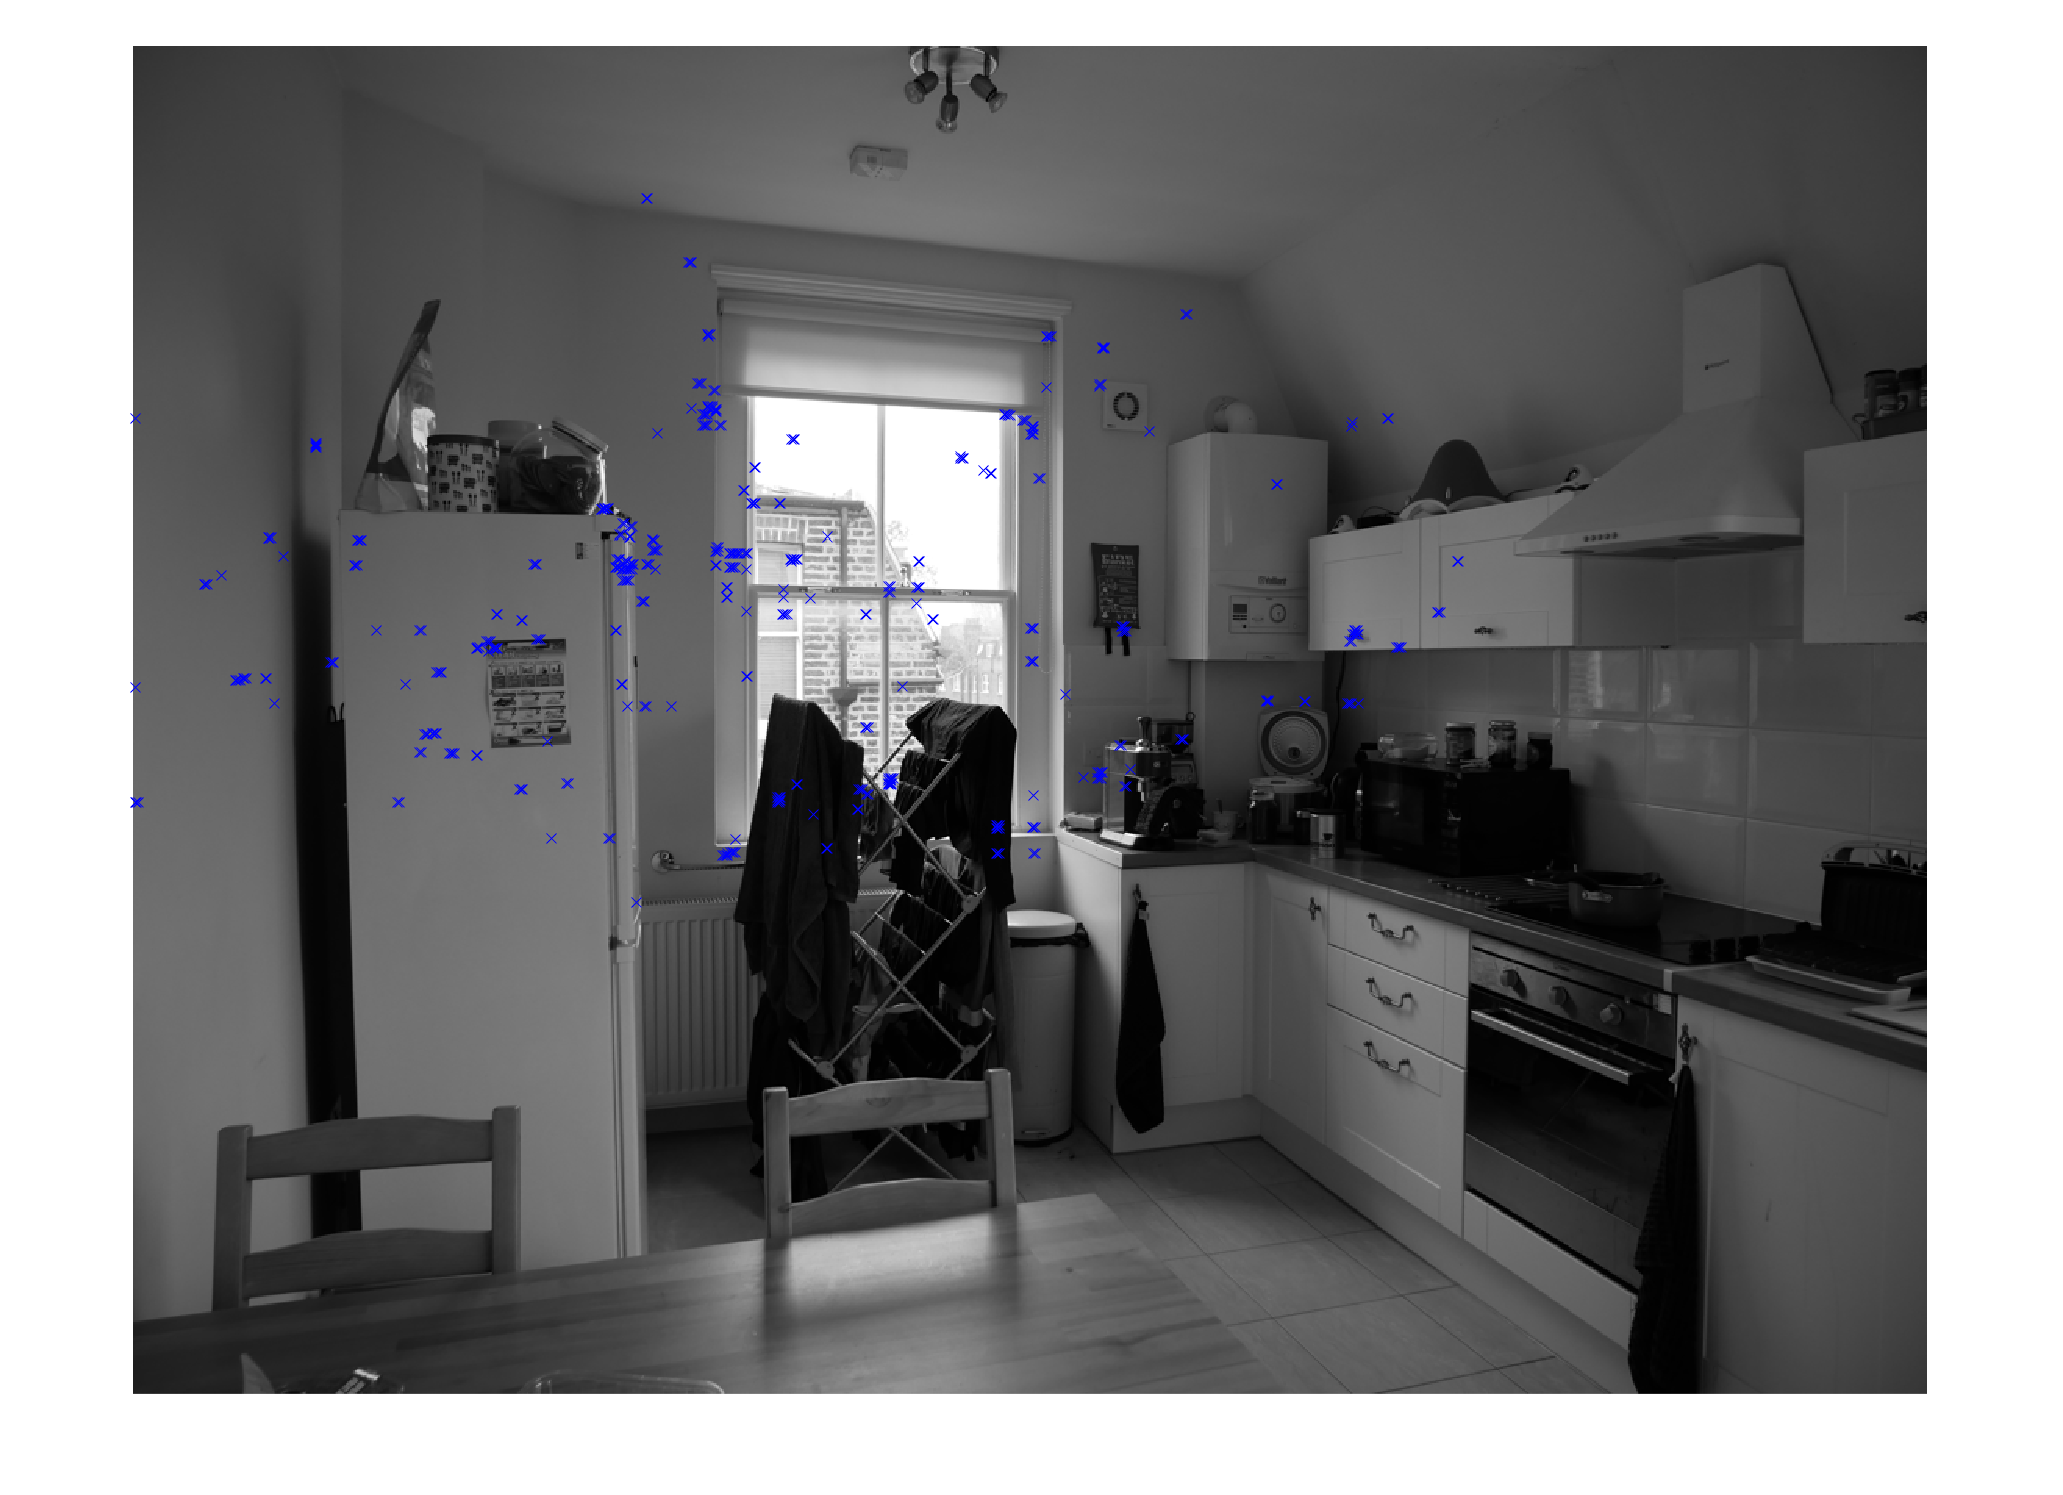
\includegraphics[width=\textwidth]{pic/hessian1e8}
      \caption{HG1 with Hessian detector, threshold $10^8$}
      \label{fig:hessian1e8}
    \end{subfigure}
    ~
    \begin{subfigure}{0.45\linewidth}
      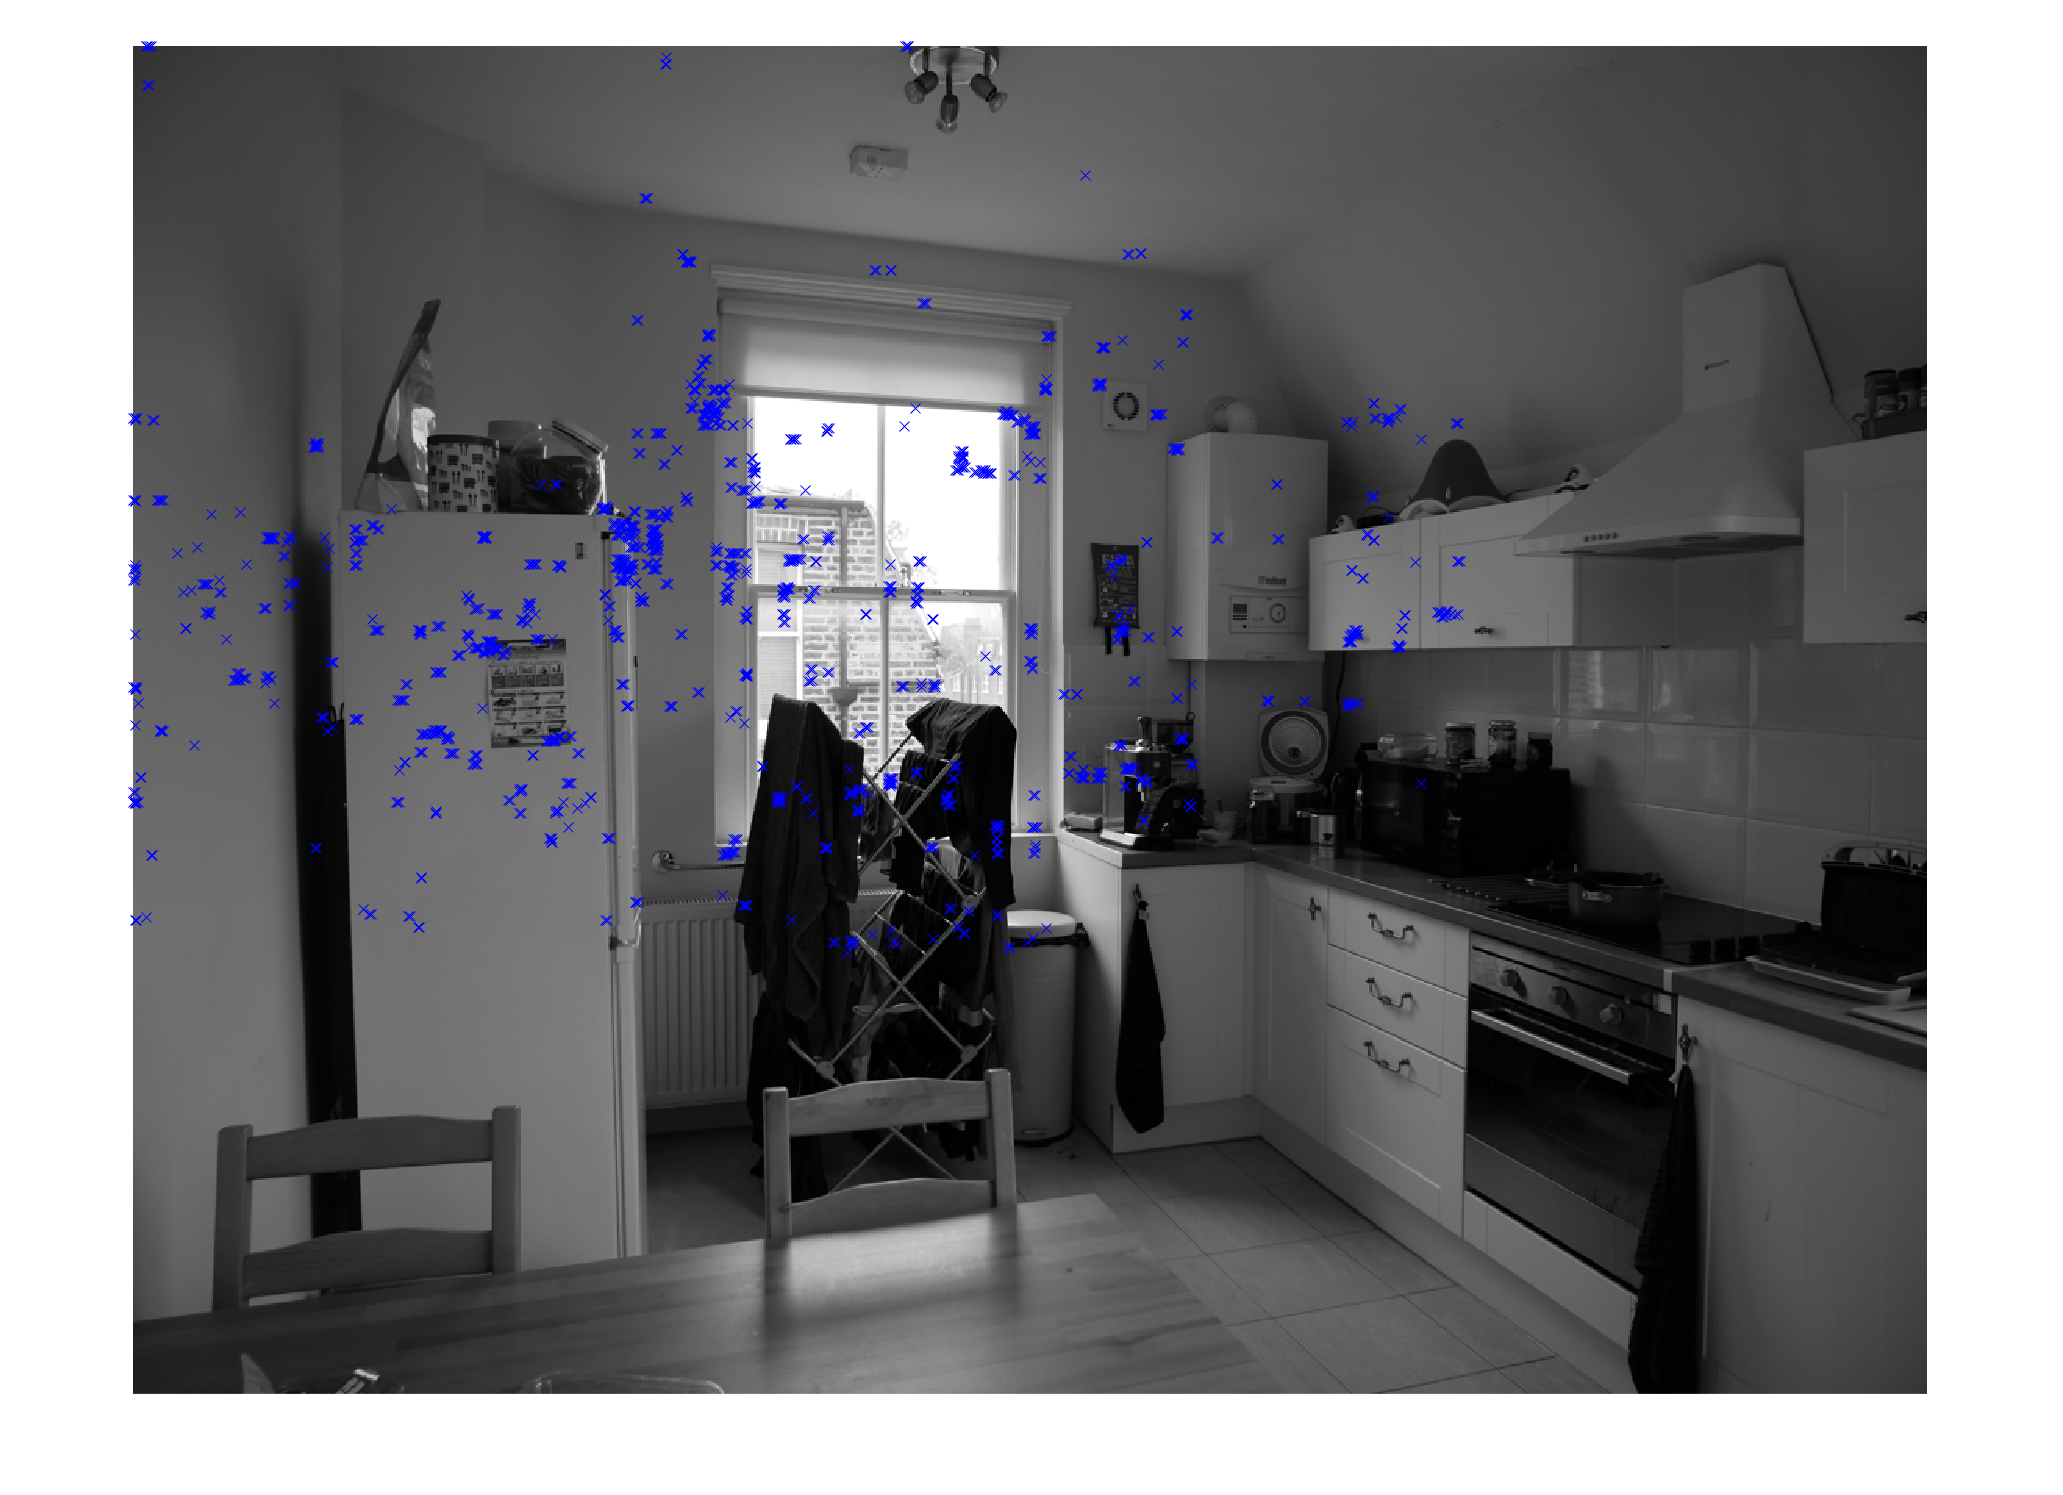
\includegraphics[width=\textwidth]{pic/harris3000}
      \caption{HG1 with Harris detector, threshold 3000}
      \label{fig:harris3000}
    \end{subfigure}

	\caption{Examples of Harris and Hessian detectors operating on Kitchen image}
    \vspace{-0.5cm}

  \label{fig:detectors}
\end{figure}

\subsubsection{Point and Patch Description}
% Discuss need for description & our implementation
Once features have been detected in the image, each point is taken as the centre of a 32x32 patch. To allow patches at the border, the image is padded by replicating the border pixels outwards (\texttt{describe.m}). The patch is then converted into a 64-bin histogram for comparison. This bin number was varied, and experimentally determined to be the most suitable for matching.

\subsubsection{Patch Matching}
% Discuss patch matching implementation - could really do with a side-by-side with lines connecting matched patches
Once each interest point has a corresponding descriptor, the points from two images are compared. Nearest Neighbour (NN) matching was used, which interprets the difference in histograms as an error, and matches the points with the least error. A match is when the two points are closest together in both directions (\texttt{matchPatches.m}).

An example image of two images with matching points is shown in Figure \ref{fig:matched}. After NN matching, the number of points has been vastly reduced and mostly correspond, with a couple of exceptions, such as the green line between the coffee pot and the coffee machine pod. These points are not the same, but the surrounding area is very similar. Those are the source of the outliers.

% I did also create this figure with showMatchedFeatures, but I found it really hard to spot where the differences are, so I did it like this. I can upload the matchedFeatures version if you want, just ask
\begin{figure}[!ht]
  \centering
  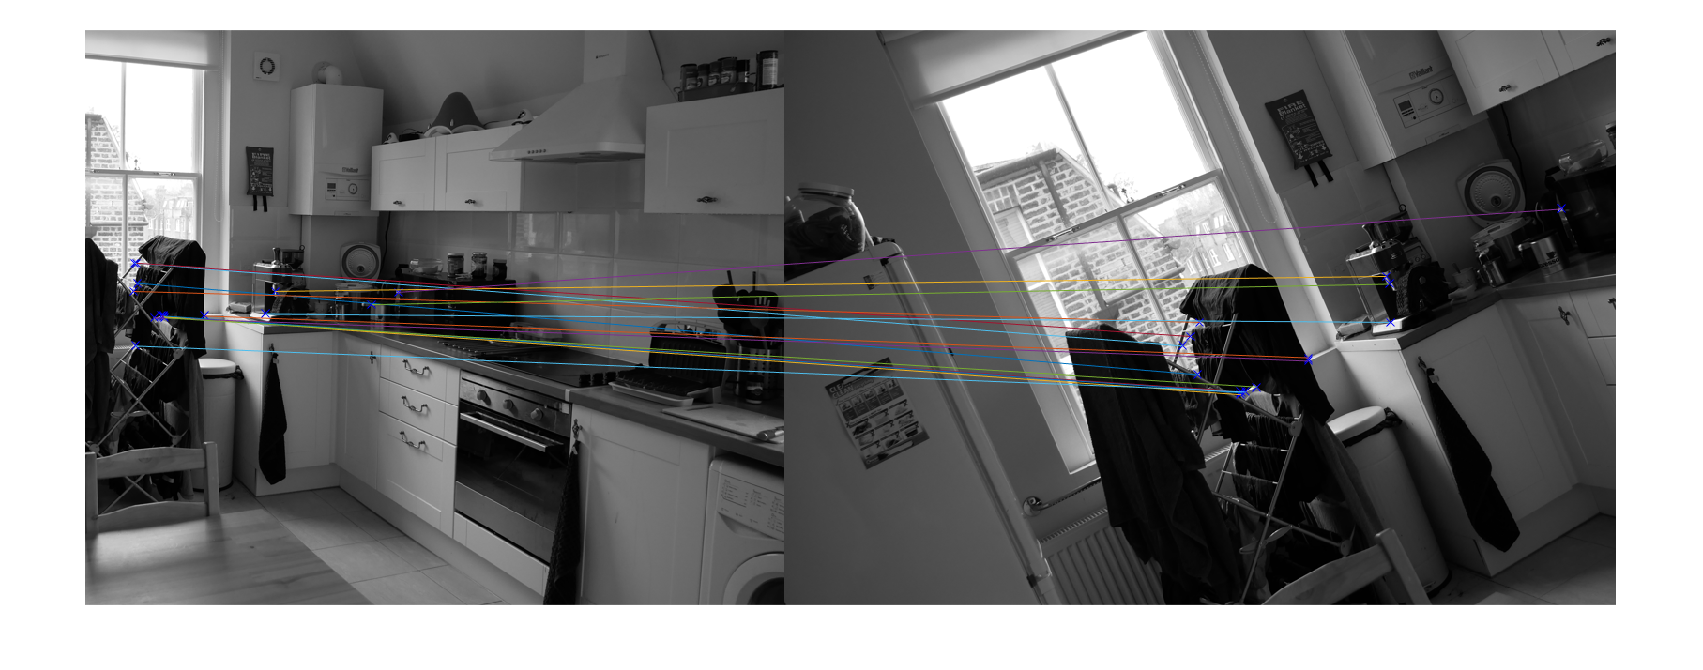
\includegraphics[width=\linewidth]{pic/matches}
  \caption{Matched patches between HG1, HG2 using Harris detector and threshold 3000}
  \vspace{-0.5cm}
  \label{fig:matched}
\end{figure}

\subsection{Transformation Estimation}

% Need to discuss homography matrix estimation and show example
\subsubsection{Homography Matrix}
The matching pairs of points can be used to estimate the transformation matrix between the two images, known as the homography matrix. The homography matrix is \textbf{H}, and must satisfy Equation \ref{eqn:homography}, where $\textbf{x}_\textbf{A}$ is the original point and $\textbf{x}_\textbf{B}$ is the destination point after the transformation. Further information on this method can be found in the course notes and lectures \cite{notes}, as well as the source file (\texttt{estTransformMat.m}).

\vspace{-0.15cm}
\begin{equation} \label{eqn:homography}
    \textbf{x}_\textbf{B} = \textbf{Hx}_\textbf{A}
\end{equation}
\vspace{-0.5cm}

%% Move from here.
\subsubsection{Homography Tranformation}
A routine was written to take the points in Image A, and project them onto the same axes as Image B (\texttt{projection.m}). Figure \ref{fig:boat13} shows the result of manually selecting points on the boat example images \cite{boat}, estimating the homography, and projecting the points through the homography matrix. While the projection method and estimation method both work well, there is slight error, shown by the green and purple parts where the images do not overlap.

\begin{figure}[!ht]
  \centering
  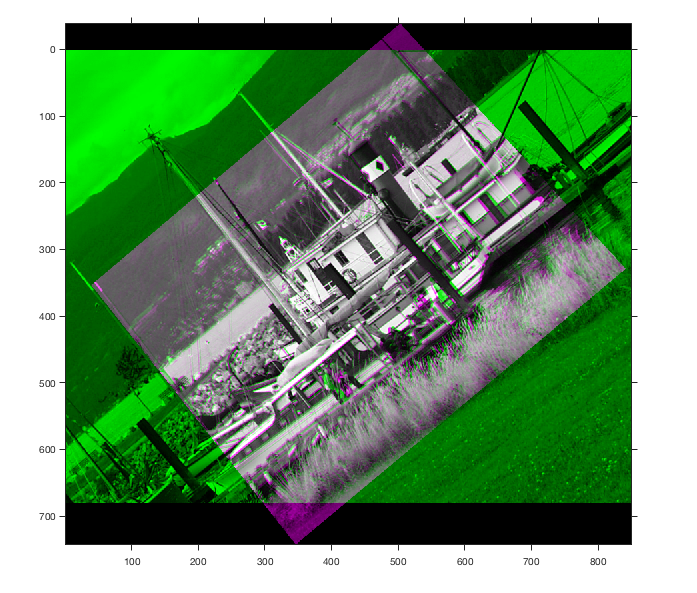
\includegraphics[width=0.75\linewidth]{pic/q2_1_b4_1_3_pair}
  \caption{Image A (Boat 1) transformed and overlaid on Image B (Boat 3)}
  \label{fig:boat13}
  \vspace{-0.5cm}
\end{figure}
%% Move end here.

% Discuss errorHA method
\subsubsection{Homography Accuracy Calculation}
To estimate how well a homography matrix matches the two sets of points together, a metric called the Homography Accuracy (HA) is used. This HA is calculated by taking the corresponding sets of points and transforming one set to fit the other using the given homography matrix. The error between the predicted and actual points is interpreted as the distance; the mean distance is the HA (\texttt{errorHA.m}. The HA for the example shown in Figure \ref{fig:boat13} is $HA=4.9149$, which is quite small.

% Need to discuss fundamental matrix estimation (and show example?)
\subsubsection{Fundamental Matrix}
Another matrix is the fundamental matrix, which can be estimated using a series of corresponding points. This matrix can be used to constrain the possible locations of points in a second image from points in the first image given the fundamental matrix between the two images. The method itself is very similar to the homography matrix, except that the relation in Equation \ref{eqn:fundamental} is used instead of that in Equation \ref{eqn:homography} (\texttt{estFundamentalMat.m}).

\vspace{-0.15cm}
\begin{equation} \label{eqn:fundamental}
    \textbf{x}_\textbf{B}^T\textbf{Fx}_\textbf{A} = 0
\end{equation}
\vspace{-0.5cm}

% Discuss epipole lines and show example
\subsubsection{Epipoles and Epipolar Lines}

The fundamental matrix means the epipole of Image A, $\textbf{e}_\textbf{A}$, can be calculated through the relationship $\textbf{Fe}_\textbf{A} = 0$. This is the intersection of every epipolar line, which means the epipolar line of each point in Image A can be found. However, more useful is the corresponding epipolar line in Image B, as that is where the corresponding point will be found. In other words, for $\textbf{x}_\textbf{A}$, $\textbf{x}_\textbf{B}$ is found on the line $\textbf{L}_\textbf{B}=\textbf{Fx}_\textbf{A}$ \cite{mit}. An example is shown in Figure \ref{fig:epipolar}. The corresponding points were manually obtained, before the fundamental matrix, epipoles, and epipolar lines were found (\texttt{epiPolesLines.m}).

\begin{figure}[!ht]
  \captionsetup[subfigure]{position=b}
  \centering
    \begin{subfigure}{0.45\linewidth}
      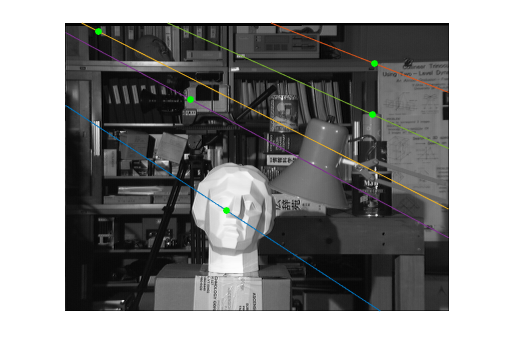
\includegraphics[width=\textwidth]{pic/q1_3_d_A}
      \caption{Tsukuba 1 as Image A  with epipole and epipolar lines.}
      \label{fig:tsuka}
    \end{subfigure}
    ~
    \begin{subfigure}{0.45\linewidth}
      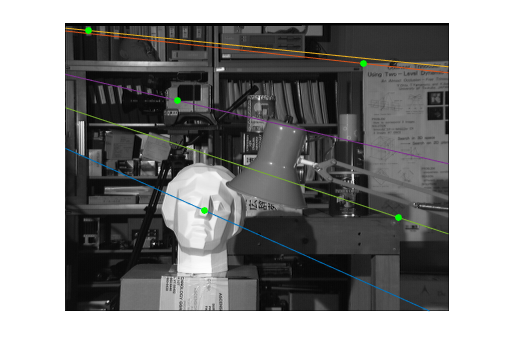
\includegraphics[width=\textwidth]{pic/q1_3_d_B}
      \caption{Tsukuba 5 as Image B with epipoles and epipolar lines.}
      \label{fig:tsukb}
    \end{subfigure}

	\caption{Epipoles and epipolar lines.}
    \vspace{-0.75cm}
  \label{fig:epipolar}
\end{figure}

\section{Question - Image Geometry}

\subsection{Homography with HG Pictures}

\subsubsection{Reduced Size}
The image HG1 was used for this test, with the Harris detector and a threshold of 500. The image was then scaled down to half its original width and height, and the same Harris detector run again. The two sets of points were matched as previously described. The HA error between the two sets of points was calculated as 0.5995. Therefore, although there are more interest points detected with the larger resolution image, the points that are matched between the two images are very close to each other. The points can be seen in Figure \ref{fig:reducedcompare}. There just appear to be more points at each cluster.

\begin{figure}[!ht]
  \centering
  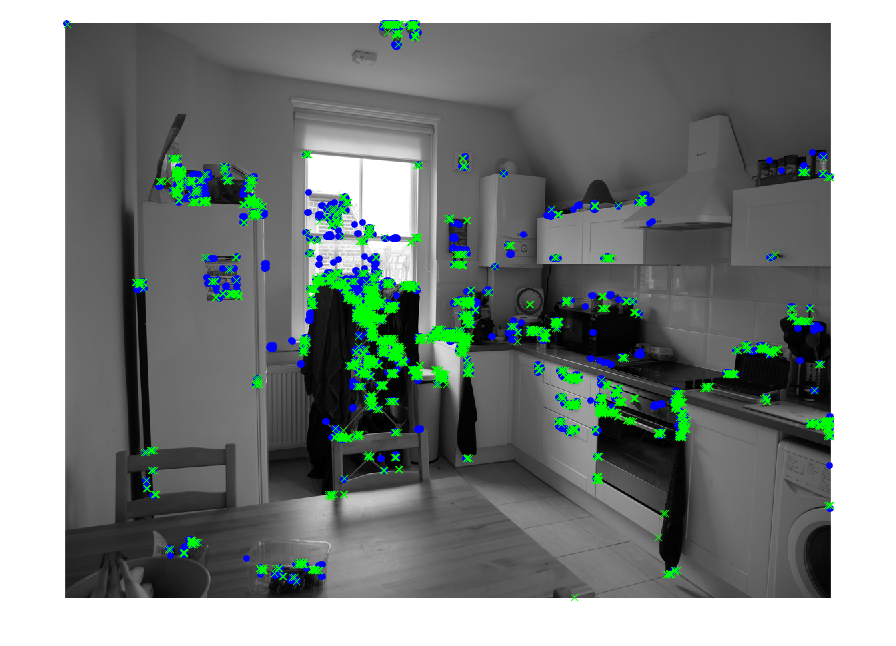
\includegraphics[width=0.75\linewidth]{pic/q2_1_a_imgBoth}
  \caption{Image HG1 with original size interest points in blue and interest points from reduced image in green.}\vspace{-.5cm}
  \label{fig:reducedcompare}
\end{figure}

\subsubsection{Manual vs. Automatic}
% Harris 4K points for 500 threshold
To evaluate automatic point detection, user-selected and automatic point selection were both used to determine the homography matrices between HG1 (A), HG2 (B), and HG3 (C). The homography from A to B, from B to C, and from C to B was first done manually. All worked as expected. Pair BC is in Figure \ref{fig:manHomog}. The success shows the effectiveness of the algorithms used. However, when the automatic detection system was used, the homography matrices were wrong. This was due to the presence of outliers. The method used to remove them is known as RANdom SAmple Consensus, or RANSAC \cite{ransac} (\texttt{myRANSAC.m}). This was run on the matching pairs before the homography estimates were done. To test this, the boat data was used again, as seen in Figure \ref{fig:boatmatches}, which shows some of the results of the automatic detection with RANSAC. The success shows the validity of our methods and functions.

\begin{figure}[!ht]
  \captionsetup[subfigure]{position=b}
  \centering
    \begin{subfigure}{0.4\linewidth}
      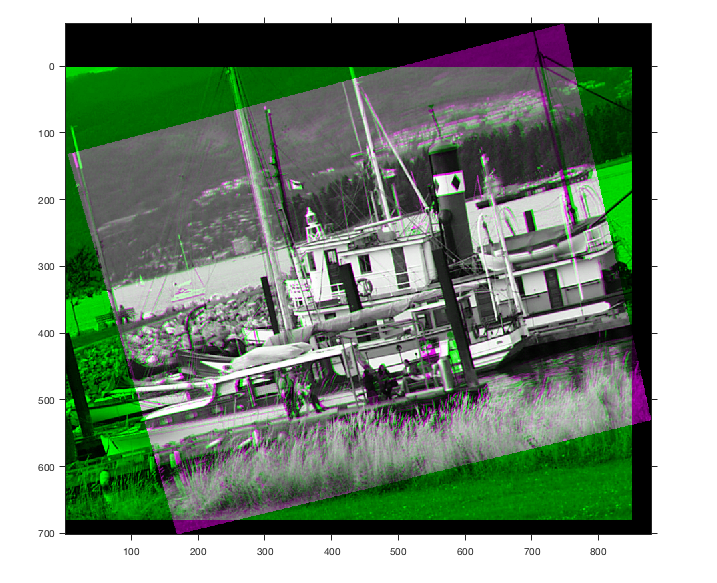
\includegraphics[width=\textwidth]{pic/q2_1_b4_1_2_pair}
      \caption{1 and 2.}
      \label{fig:boatmatch12}
    \end{subfigure}
    ~
    \begin{subfigure}{0.4\linewidth}
      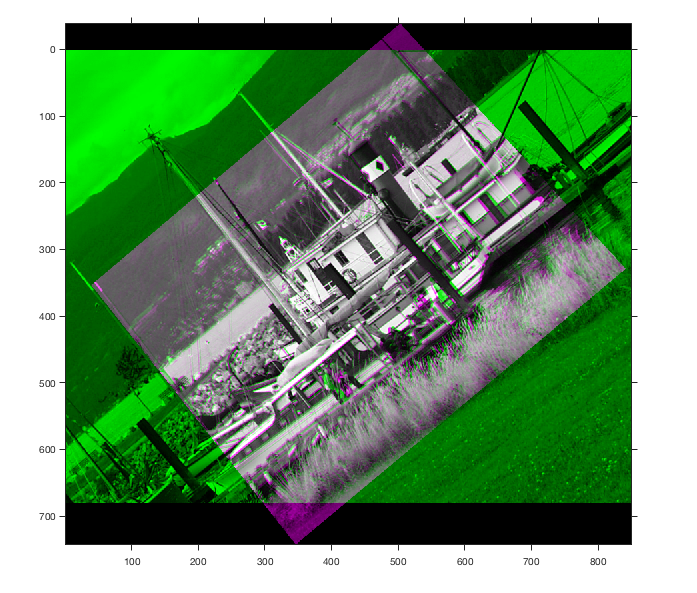
\includegraphics[width=\textwidth]{pic/q2_1_b4_1_3_pair}
      \caption{1 and 3.}
      \label{fig:boatmatch13}
  \end{subfigure}
  \\
  \begin{subfigure}{0.4\linewidth}
    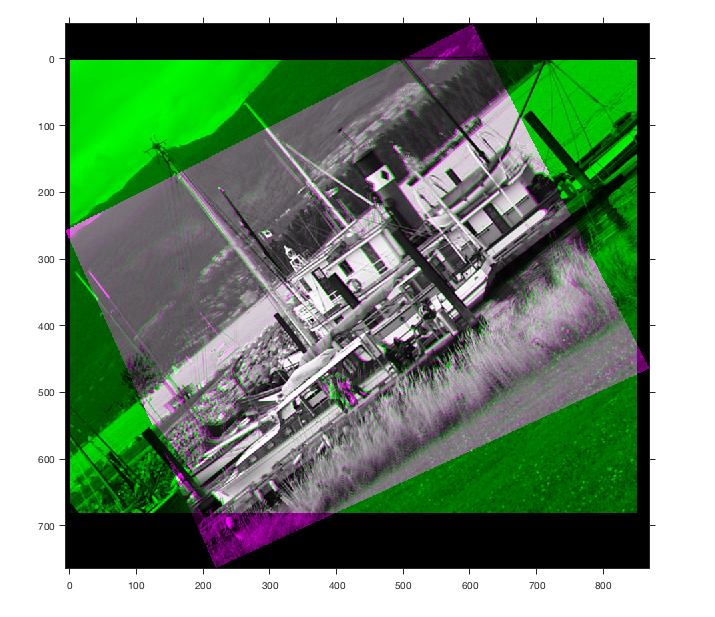
\includegraphics[width=\textwidth]{pic/q2_1_b4_2_3_pair}
    \caption{2 and 3.}
    \label{fig:boatmatch23}
  \end{subfigure}
  ~
  \begin{subfigure}{0.4\linewidth}
    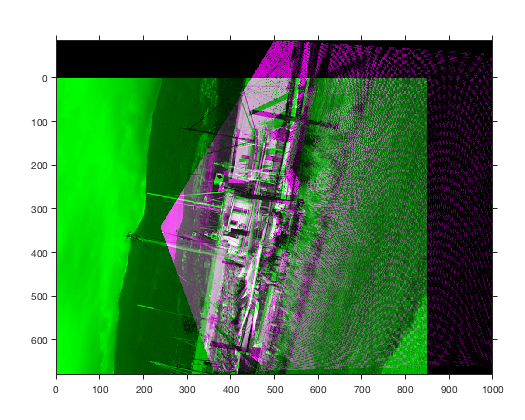
\includegraphics[width=\textwidth]{pic/q2_1_b4_3_4_pair}
    \caption{3 and 4.}
    \label{fig:boatmatch34}
\end{subfigure}
	\caption{HG results for boat with RANSAC.}
    \vspace{-0.5cm}
  \label{fig:boatmatches}
\end{figure}

However, when the same method was applied to our pictures, only the BC pair worked, in Figure \ref{fig:autoHomog}. To attempt to confirm the error in the algorithm, MATLAB's Harris methods were used as reference. MATLAB was able to work out the AB pair, but neither the BC nor the CA pair! In contrast, the SURF methods of MATLAB were able to work out all 3 pairs. Our methods had a success rate of 33\%, on par with the MATLAB methods. Combining this observation with the success of the boat photos suggests that the Harris detection was not suitable for the HG photos. The image results from the MATLAB methods are found in the Appendix.

% Need to show automatic vs. manual for a pair of pictures
% Need to visualise those homographies
% Need to analyse those homographies for translation/rotation/projection things

The matrices $\textbf{H}_{man}$ and $\textbf{H}_{auto}$ represent the homography matrices estimated from user-selected points and Harris-detected points, respectively. These transformations are also visualised in Figure \ref{fig:matchBC}, which shows that $\textbf{H}_{man}$ is closer to the true matrix, as the edges and objects within the images line up more closely and there is less blur.

% Select pair B->C as it is the only working pair

\begin{equation} \label{eqn:manHomog}
\textbf{H}_{man} = \begin{bmatrix}
     1.5542 &  0.5391 & -533.90 \\
    -0.5575 &  1.5585 &  92.584 \\
    -0.0000 &  0.0000 &  1.0000
\end{bmatrix}
\end{equation}

\begin{equation} \label{eqn:autoHomog}
\textbf{H}_{auto} = \begin{bmatrix}
     1.7543 &  0.6687 & -645.30 \\
    -0.5892 &  1.8003 &  47.431 \\
     0.0000 &  0.0001 &  1.0000
\end{bmatrix}
\end{equation}

These matrices can be analysed as similarity matrices, yielding a scale factor change, a rotation, and a translation \cite{notes}. The $<x, y>$ translation are given by $h_{13}$ and $h_{23}$ of each matrix; there seems to be a significant difference between the two. As the scale and rotation are multiples, these are more complex to compute. A script was used to compute the scale factor from the mean of the sine terms and the mean of the cosine terms, adjusting the angle until the two scale factors are close. This computation shows that $\textbf{H}_{auto}$ has a rotation of 19.49\degree, and a scale factor of 1.885; $\textbf{H}_{man}$ has a rotation of 21.5\degree, and a scale factor of 1.67. As the camera was rotated by 20\degree, and zoomed by 1.5, this latter matrix represents the transformation better.

\begin{figure}[!ht]
  \captionsetup[subfigure]{position=b}
  \centering
    \begin{subfigure}{0.45\linewidth}
      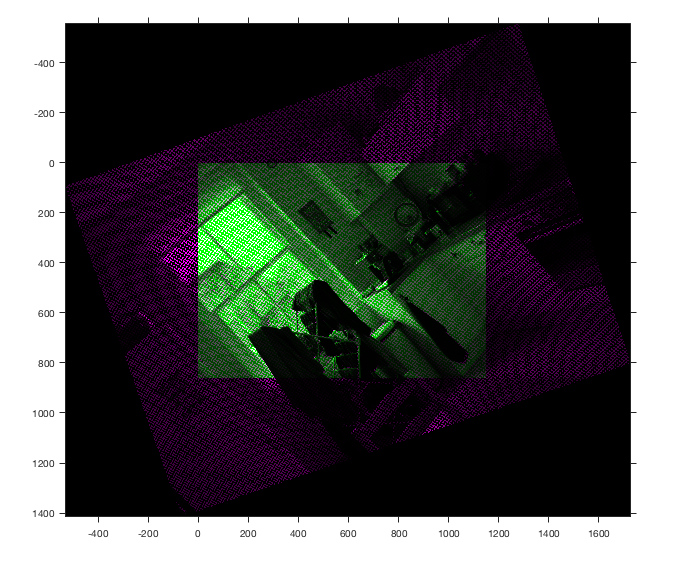
\includegraphics[width=\textwidth]{pic/q2_1_b1_BC_pair}
      \caption{$\textbf{H}_{man}$ matrix}
      \label{fig:manHomog}
    \end{subfigure}
    ~
    \begin{subfigure}{0.45\linewidth}
      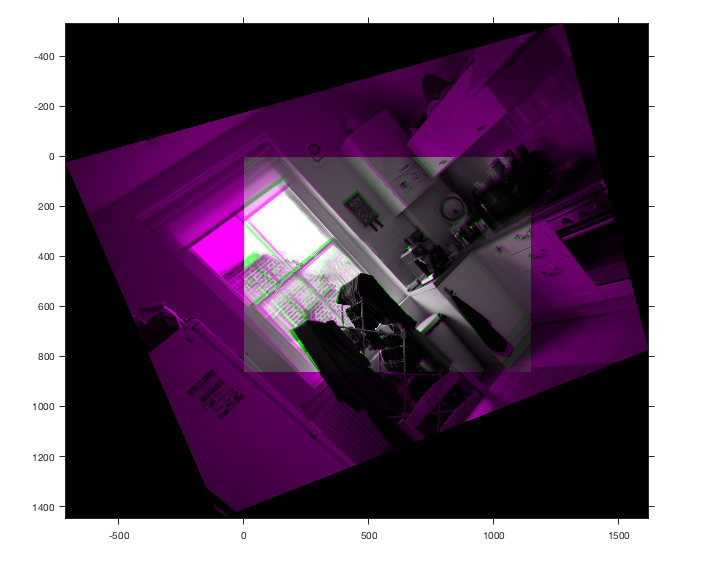
\includegraphics[width=\textwidth]{pic/q2_1_b2_BC_pair}
      \caption{$\textbf{H}_{auto}$ matrix}
      \label{fig:autoHomog}
    \end{subfigure}

	\caption{Transformation given by homography matrix between images B and C, with B in purple and C in green}
    \vspace{-0.5cm}

  \label{fig:matchBC}
\end{figure}


\subsubsection{Number of Correspondences}

% Need to go through a few different numbers of correspondences and see how the homography changes
% Find the number of outliers
% Explain how you found the outliers

% TODO what was the result of these tests?
For the pair BC that worked, the original number of matches was 439. The number of inliers was 278; the number of outliers was 161. As discussed, RANSAC was used to remove the outliers. The number of inlier points was considered and between 4 and 278 were randomly selected to calculate the homography matrix, before the HA was calculated. The result is shown in Figure \ref{fig:outliers}. The error is low and constant at high numbers. The error spikes heavily as this decreases, but drops when there are very few points. In other words, the post-RANSAC selection of points still contains some outliers, but they are much rarer than before. However, once a certain subset of the post-RANSAC points are selected, there is a higher chance that a selection will contain more outliers that the homography estimation can cope with. At small numbers, the chances of selecting only the valid points are higher, hence the lower error.

\begin{figure}[!ht]
  \centering
  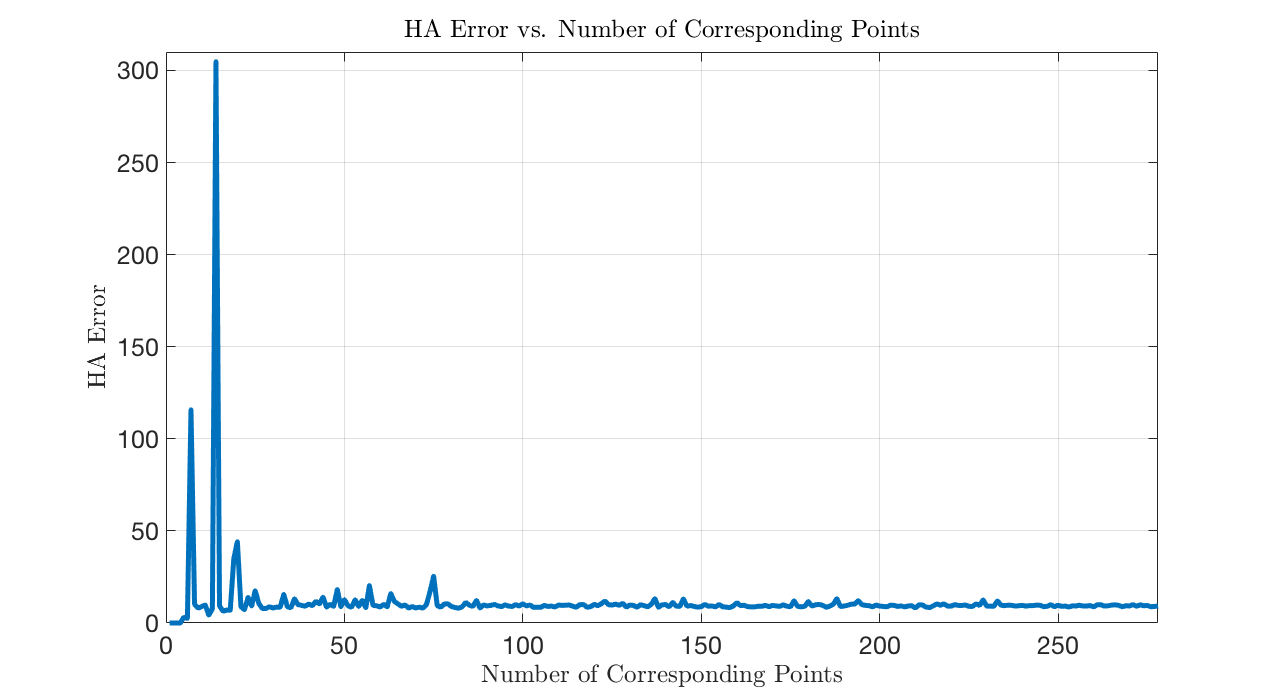
\includegraphics[width=0.75\linewidth]{pic/q2_1_c}
  \caption{Graphs of HA against number of corresponding points}
  \vspace{-0.5cm}
  \label{fig:outliers}
\end{figure}

\subsection{Stereo Vision With FD Pictures}
\subsubsection{Epipoles and Epipolar Lines}

% Estimate fundamental matrix from manual points with FD pics
% Calculate epipoles for A,B and show

For each pair FD1 and FD2, FD2 and FD3, FD3 and FD1, the fundamental matrix is estimated and the epipoles and epipolar lines calculated. The epipolar lines and epipoles for the FD1, FD2 pair are given in Figure \ref{fig:fdEpipoles}, with the matrix estimated in Equation \ref{eqn:fundamentalFD}. The near-horizontal lines suggest that the photos are almost coplanar, and this is reasonable as the camera was moved only horizontally for the FD images.

\begin{equation} \label{eqn:fundamentalFD}
\textbf{F} = \begin{bmatrix}
     0.0000 & -0.0000 &  0.0234 \\
     0.0000 &  0.0000 & -0.1198 \\
    -0.0259 &  0.1235 &  1.0000
\end{bmatrix}
\end{equation}

\begin{figure}[!ht]
  \centering
  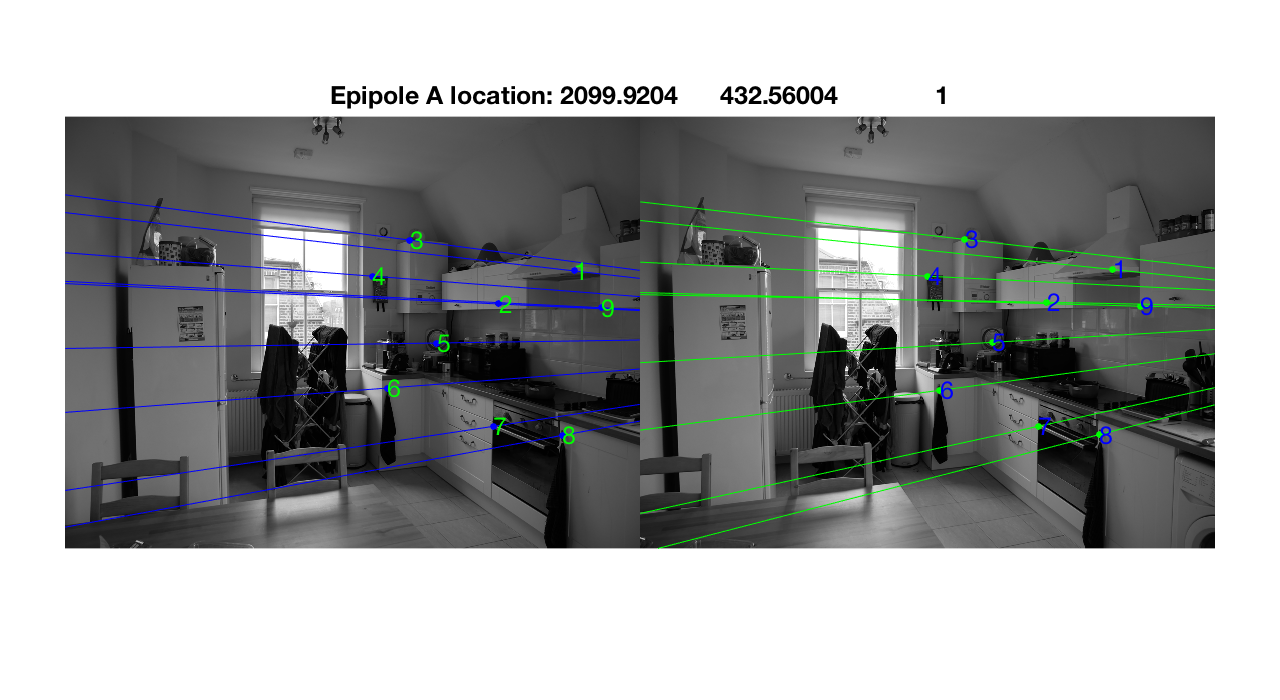
\includegraphics[width=0.75\linewidth]{pic/q2_2_ab_A_0}
  \caption{Epipoles and epipolar lines between images FD1 and FD2}
  \vspace{-0.5cm}
  \label{fig:fdEpipoles}
\end{figure}

\subsubsection{Disparity}

To calculate disparity, the method of Sum Squared Differences (SSD) was used. FD1 (A) is split into windows, and the most similar window in searched for in FD2 (B). The difference in $x$ values of the centers of the window in A and the matching window in B is the disparity. To reduce the amount of searching, the points selected in B for comparison are limited to those on the epipolar line in B corresponding to the centre of the window in A. However, if the pictures are coplanar, the method may not be as effective as the search should happen along the horizontal line, even if the calculated epipolar lines are not parallel. To test this, the Tsukuba data was used again, shown in Figure \ref{fig:q2_2_cd_tkb}. It shows that if the pictures are coplanar, even if the calculated epipolar lines are not parallel, using parallel horizontal lines yields better results. As such, for A and B, only horizontal lines were searched, as the camera was only moved horizontally. The disparity map is shown in \ref{fig:depth10}. However, the Tsukuba example shows proof that an epipolar line search method was written and would work for other non-coplanar pictures.

\begin{figure}[!ht]
  \captionsetup[subfigure]{position=b}
  \centering
    \begin{subfigure}{0.45\linewidth}
      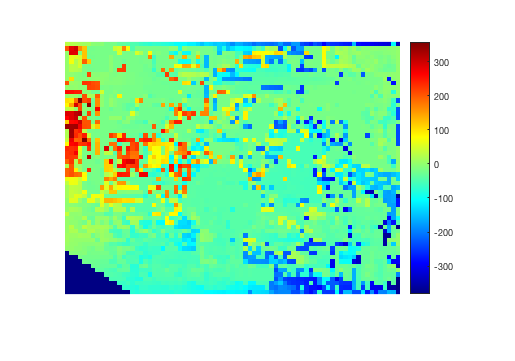
\includegraphics[width=\textwidth]{pic/q2_2_cd1_dis}
      \caption{Epipolar lines.}
      \label{fig:q2_2_cd1_tkb}
    \end{subfigure}
    ~
    \begin{subfigure}{0.45\linewidth}
      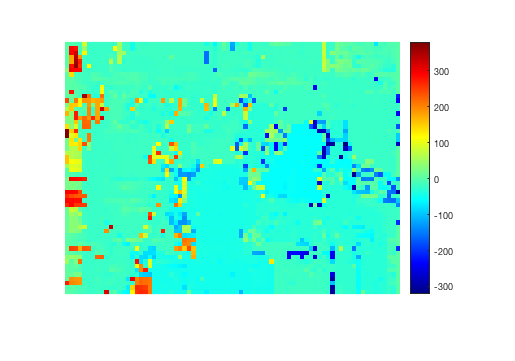
\includegraphics[width=\textwidth]{pic/q2_2_cd2_dis}
      \caption{Horizontal lines.}
      \label{fig:q2_2_cd3_tkb}
    \end{subfigure}

	\caption{Comparison of disparity calculation along epipolar lines and along horizontal lines for Tsukuba data. }
    \vspace{-0.5cm}
  \label{fig:q2_2_cd_tkb}
\end{figure}

\begin{figure}[!ht]
  \captionsetup[subfigure]{position=b}
  \centering
    \begin{subfigure}{0.45\linewidth}
        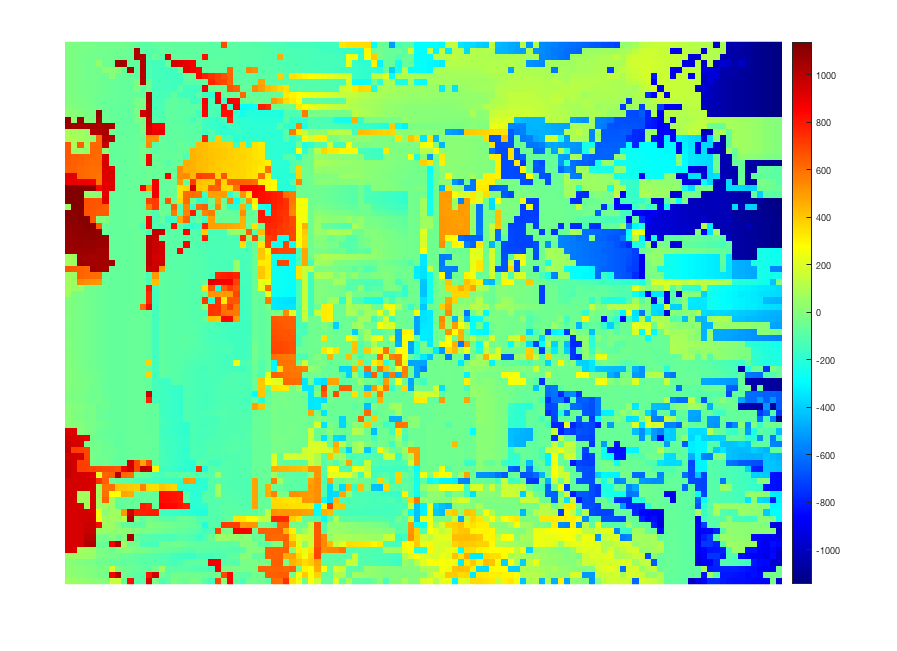
\includegraphics[width=\linewidth]{pic/q2_2_cd4_dis}
        \caption{Disparity map.}
        \label{fig:depth10}
    \end{subfigure}
    ~
    \begin{subfigure}{0.45\linewidth}
        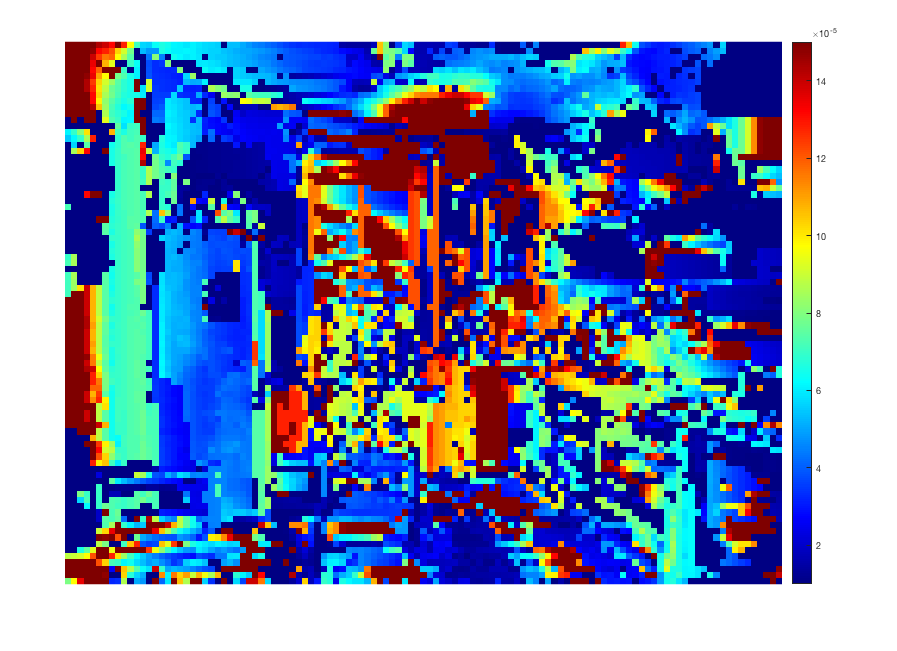
\includegraphics[width=\linewidth]{pic/q2_2_cd4_depth}
      	\caption{Depth map. $f = 24\text{mm}$, $b = 20\text{cm}$.}
        \label{fig:depth}
    \end{subfigure}

	\caption{FD1 using FD2, with 10x10 window size. Using horizontal lines.}
    \vspace{-0.5cm}
  \label{fig:q2_2_cd_4}
\end{figure}


\subsubsection{Depth}

To convert from disparity to depth ($z$), the formula $z = \frac{fb}{d}$, where $f$ is the focal length, $b$ is the baseline, and $d$ is the disparity. The absolute value of the disparity was taken as there cannot be negative distance. Figure \ref{fig:depth} shows this. The window size was empirically chosen for the best result. The results are as expected, with the red portions (a higher depth) being mostly in the centre, around the window and the far side of the kitchen. The left and right parts of the image should be closer, and there is more blue, but there are outliers. A large patch of red is on the left, as is a light green one. The fridge is surprisingly blue. Upon closer inspection, the picture does have a lot of uniform white areas (wall, ceiling, fridge), which may have caused issues with feature recognition in earlier segments as well. However, this is again the result of the image, rather than the method, as evidenced by the success of the identical code with the Tsukuba data.

\subsubsection{Focal Length and Noise}

The depth map was calculated again, with $f = 22\text{mm}$, then with $f = 26\text{mm}$ and finally with $f = 24\text{mm}$ again, but adding Gaussian noise to the disparity map. Increasing the focal length should make everything further away, and reducing it vice-versa. This is visible as a slight shift to red in Figure \ref{fig:q2_2_e_focal1}, and more blue in Figure \ref{fig:q2_2_e_focal2}. However, this was very little. Adding noise shown in Figure \ref{fig:q2_2_e_gaussian} appears to have no effect, whether at small or large amounts, as it either has no visible effort, or simply makes the depth map filled with artefacts.

\begin{figure}[!ht]
  \captionsetup[subfigure]{position=b}
  \centering
    \begin{subfigure}{0.45\linewidth}
      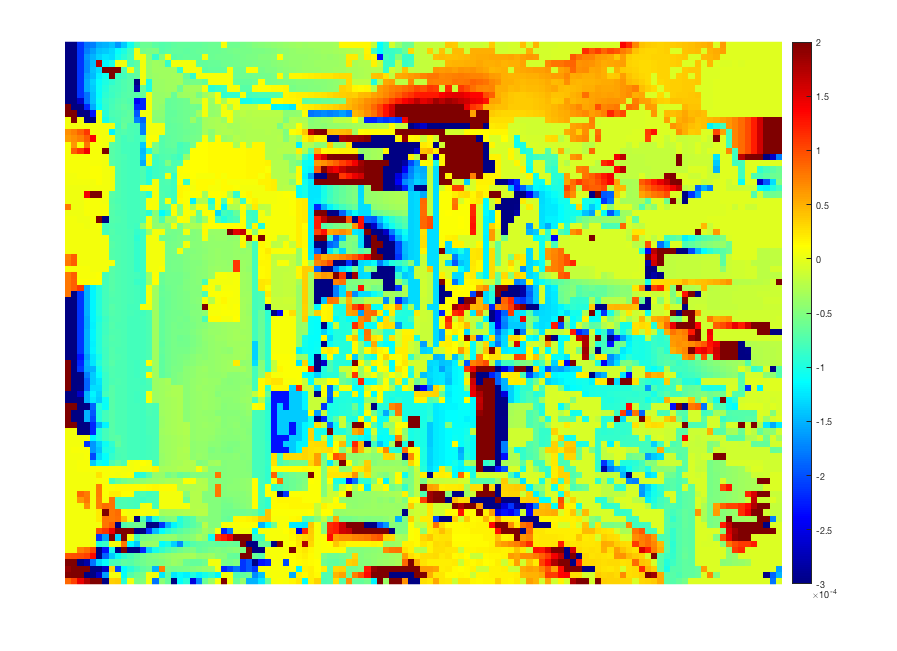
\includegraphics[width=\textwidth]{pic/q2_2_e_focal1}
      \caption{$f = 26\text{mm}$}
      \label{fig:q2_2_e_focal1}
    \end{subfigure}
    ~
    \begin{subfigure}{0.45\linewidth}
      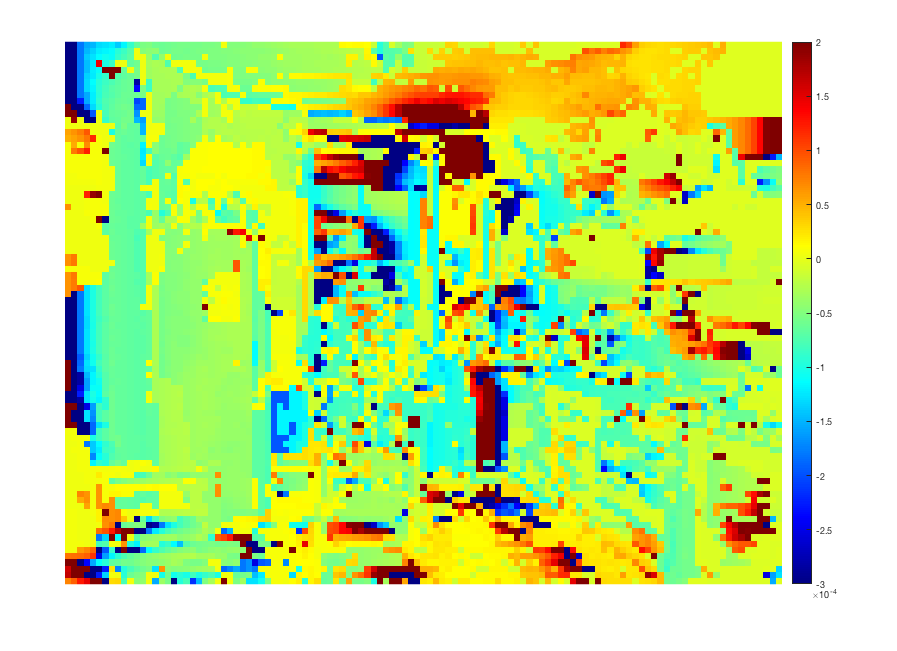
\includegraphics[width=\textwidth]{pic/q2_2_e_focal2}
      \caption{$f = 22\text{mm}$}
      \label{fig:q2_2_e_focal2}
    \end{subfigure}

    \caption{Depth map for FD1 using FD2, with 10x10 window size. $f = 24\text{mm}$, $b = 20\text{cm}$.}
    \vspace{-0.5cm}
  \label{fig:q2_2_e_focal}
\end{figure}

\begin{figure}[!ht]
  \centering
  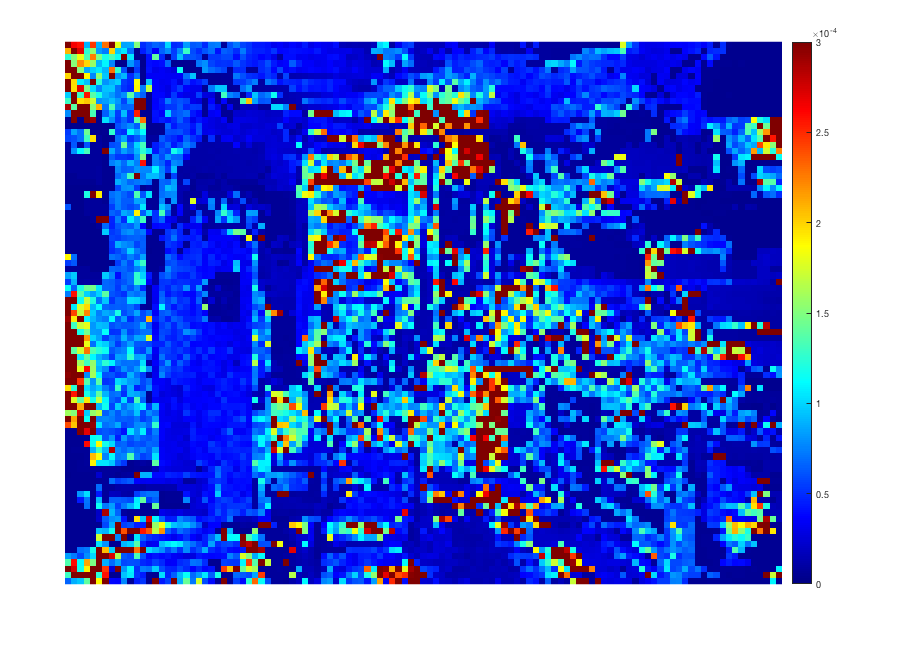
\includegraphics[width=0.75\linewidth]{pic/q2_2_e_gaussian}
	\caption{Depth map for FD1 using FD2, with $\sigma = 16$, capped at $\pm 50$.}
    \vspace{-0.5cm}
  \label{fig:q2_2_e_gaussian}
\end{figure}


%-------------------------------------------------------------------------------
% Conclusion
%-------------------------------------------------------------------------------
% \section{Conclusion}
% Lorem ipsum dolor sit amet, consectetur adipiscing elit. Phasellus gravida viverra sollicitudin. Nulla ornare enim in ante auctor rhoncus a vel nulla. Nulla condimentum massa rhoncus, sodales arcu a, euismod nulla. Proin viverra mauris at massa molestie, a ultricies tortor fermentum. Duis consectetur, ante a tincidunt euismod, augue diam varius dolor, ut vestibulum orci est sit amet mi.

%-------------------------------------------------------------------------------
% References
%-------------------------------------------------------------------------------
\bibliographystyle{unsrt}
\bibliography{mlcv_refs}

%-------------------------------------------------------------------------------
% Appendix(ces)
%-------------------------------------------------------------------------------
\onecolumn
\section*{Appendix}

\subsection*{q1\_manual.m}
\lstinputlisting[style=Matlab-editor]{src/q1_manual.m}
\newpage

\subsection*{hessian.m}
\lstinputlisting[style=Matlab-editor]{src/hessian.m}
\newpage

\subsection*{harris.m}
\lstinputlisting[style=Matlab-editor]{src/harris.m}
\newpage

\subsection*{describe.m}
\lstinputlisting[style=Matlab-editor]{src/describe.m}
\newpage

\subsection*{matchPatches.m}
\lstinputlisting[style=Matlab-editor]{src/matchPatches.m}
\newpage

\subsection*{estTransformMat.m}
\lstinputlisting[style=Matlab-editor]{src/estTransformMat.m}
\newpage

\subsection*{estFundamentalMat.m}
\lstinputlisting[style=Matlab-editor]{src/estFundamentalMat.m}
\newpage

\subsection*{projection.m}
\lstinputlisting[style=Matlab-editor]{src/projection.m}
\newpage

\subsection*{errorHA.m}
\lstinputlisting[style=Matlab-editor]{src/errorHA.m}
\newpage

\subsection*{epiPolesLines.m}
\lstinputlisting[style=Matlab-editor]{src/epiPolesLines.m}
\newpage

\subsection*{Code for Q.1.3.d}

\begin{figure}[!ht]
  \captionsetup[subfigure]{position=b}
  \centering
    \begin{subfigure}{0.45\linewidth}
      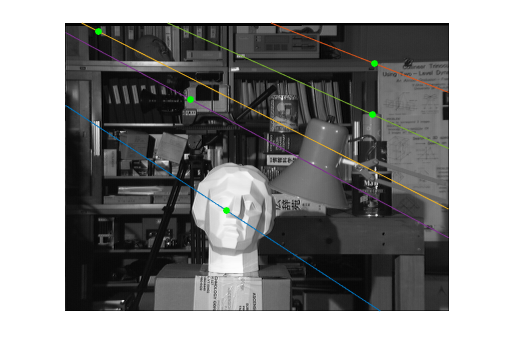
\includegraphics[width=\textwidth]{pic/q1_3_d_A}
      \caption{Tsukuba 1 as Image A  with epipole and epipolar lines.}
    \end{subfigure}
    ~
    \begin{subfigure}{0.45\linewidth}
      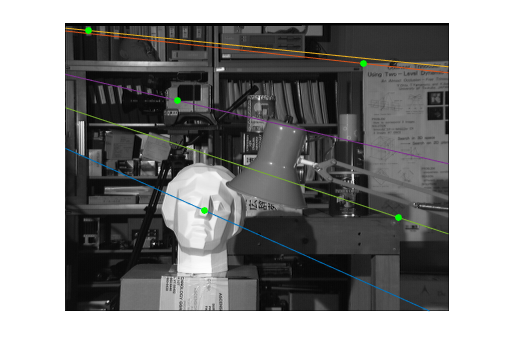
\includegraphics[width=\textwidth]{pic/q1_3_d_B}
      \caption{Tsukuba 5 as Image B with epipoles and epipolar lines.}
    \end{subfigure}

	\caption{Epipoles and epipolar lines.}
\end{figure}

\lstinputlisting[style=Matlab-editor]{src/q1_3_d.m}
\newpage

\subsection*{Code for Q2.1.a}

\begin{figure}[!ht]
  \centering
  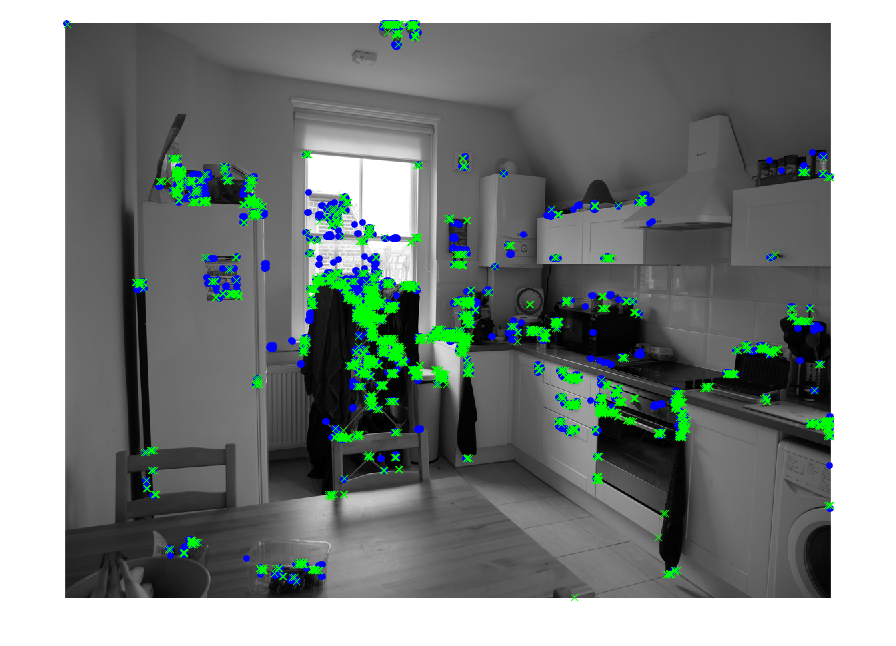
\includegraphics[width=\linewidth]{pic/q2_1_a_imgBoth}
  \caption{Image HG1 with original size interest points in blue and interest points from reduced image in green.}
\end{figure}

\lstinputlisting[style=Matlab-editor]{src/q2_1_a.m}
\newpage

\subsection*{myRANSAC.m}

\subsubsection{Method Description}
\begin{enumerate}
    \item Randomly select minimum number of points from data set to form the model. In this case, 4.
    \item Calculate model. Measure deviation from model of each point in data set.
    \item Find the subset that lies within a specified margin of the model. Measure the size of that subset.
    \item Repeat 1. and 2. as many times as desired.
    \item Keep the largest subset from all the iterations. These are the inliers.
\end{enumerate}

\lstinputlisting[style=Matlab-editor]{src/myRANSAC.m}
\newpage

\subsection*{Code for Q2.1.b. Initial point detection and generation were skipped when using manual points.}

\begin{figure}[!ht]
  \captionsetup[subfigure]{position=b}
  \centering
    \begin{subfigure}{0.3\linewidth}
      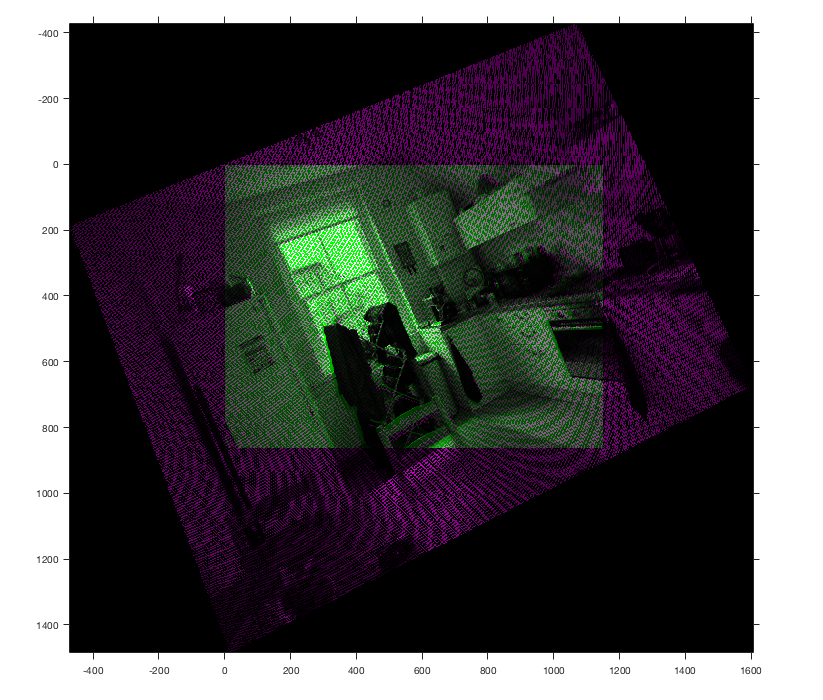
\includegraphics[width=\textwidth]{pic/q2_1_b1_AB_pair}
      \caption{A and B.}
    \end{subfigure}
    ~
    \begin{subfigure}{0.3\linewidth}
      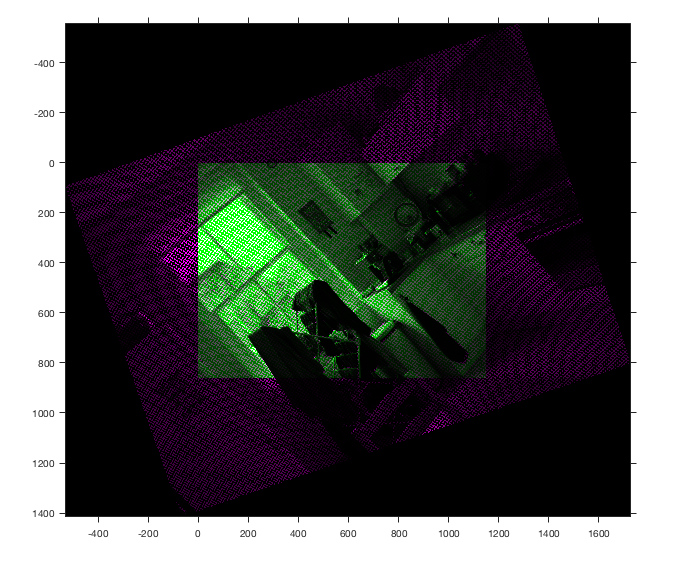
\includegraphics[width=\textwidth]{pic/q2_1_b1_BC_pair}
      \caption{B and C.}
    \end{subfigure}
    ~
    \begin{subfigure}{0.3\linewidth}
      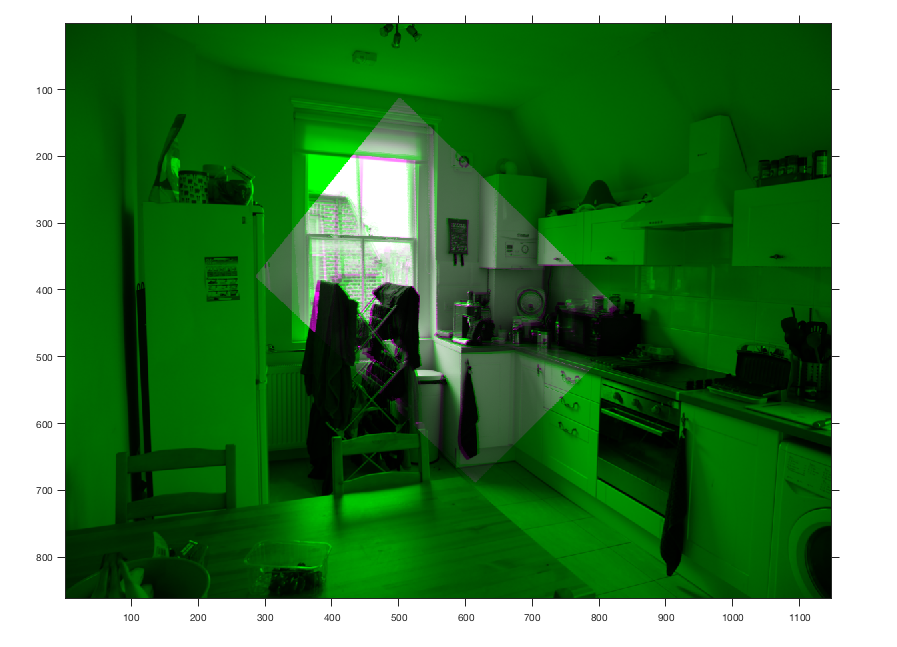
\includegraphics[width=\textwidth]{pic/q2_1_b1_CA_pair}
      \caption{C and A.}
    \end{subfigure}

	\caption{HG Matching Pairs with Manual Points.}
\end{figure}

\lstinputlisting[style=Matlab-editor]{src/q2_1_b2.m}
\newpage

\subsection*{Code for Q2.1.b with SURF Features. For MATLAB Harris features, \texttt{detectHarrisFeatures} was used instead.}

\begin{figure}[!ht]
  \captionsetup[subfigure]{position=b}
  \centering
    \begin{subfigure}{0.3\linewidth}
      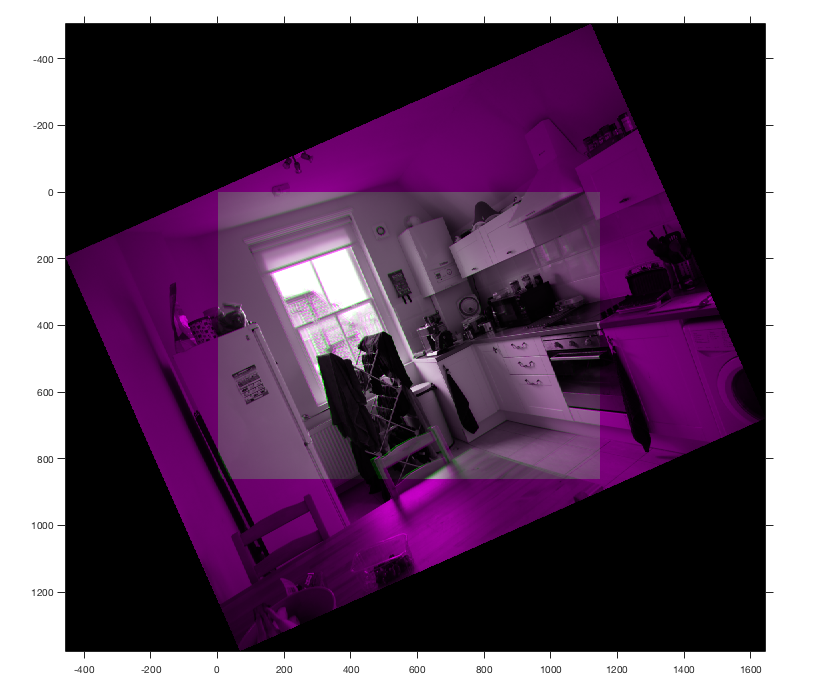
\includegraphics[width=\textwidth]{pic/q2_1_b5_AB}
      \caption{A and B.}
    \end{subfigure}
    ~
    \begin{subfigure}{0.3\linewidth}
      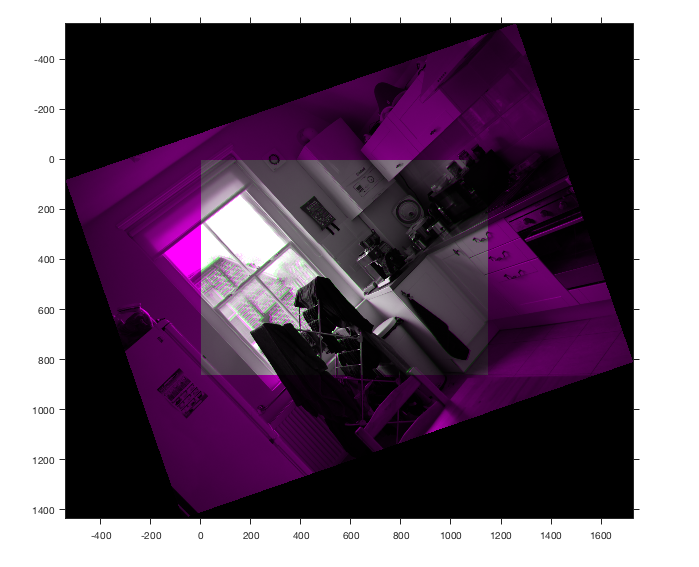
\includegraphics[width=\textwidth]{pic/q2_1_b5_BC}
      \caption{B and C.}
    \end{subfigure}
    ~
    \begin{subfigure}{0.3\linewidth}
      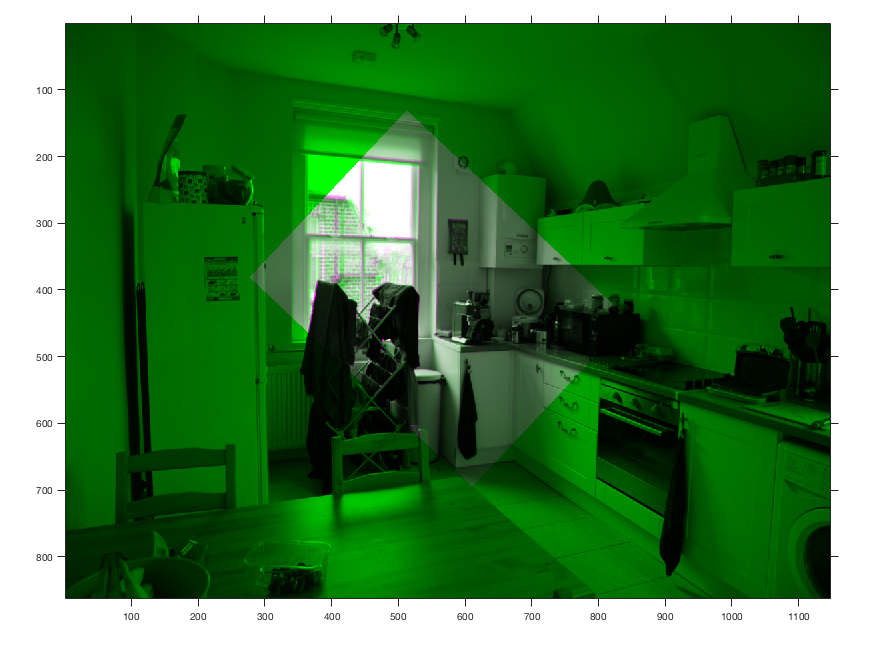
\includegraphics[width=\textwidth]{pic/q2_1_b5_CA}
      \caption{C and A.}
    \end{subfigure}

	\caption{HG Matching Pairs with SURF.}
\end{figure}

\lstinputlisting[style=Matlab-editor]{src/q2_1_b5.m}
\newpage

\subsection*{Code for Q2.1.c}

\begin{figure}[!ht]
  \centering
  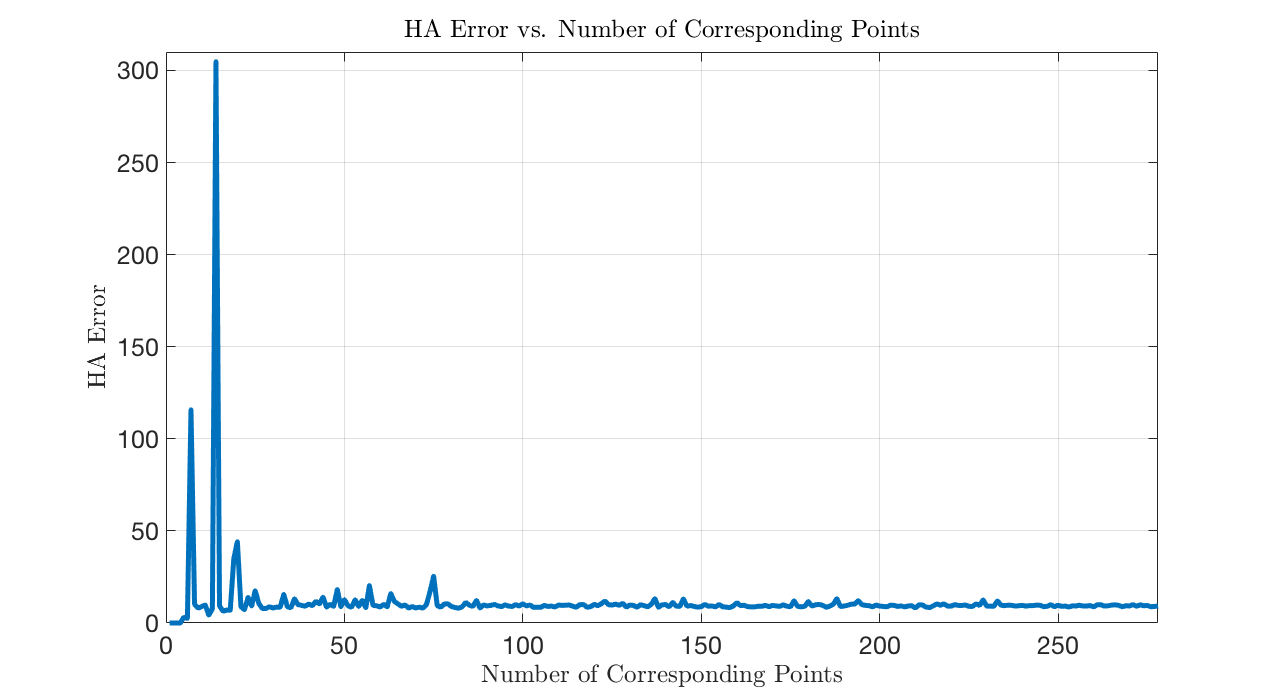
\includegraphics[width=\linewidth]{pic/q2_1_c}
  \caption{Graphs of HA against number of corresponding points}
\end{figure}

\lstinputlisting[style=Matlab-editor]{src/q2_1_c.m}
\newpage

\subsection*{Code for Q2.2.a and Q2.2.b}

\begin{figure}[!ht]
  \captionsetup[subfigure]{position=b}
  \centering
    \begin{subfigure}{0.45\linewidth}
        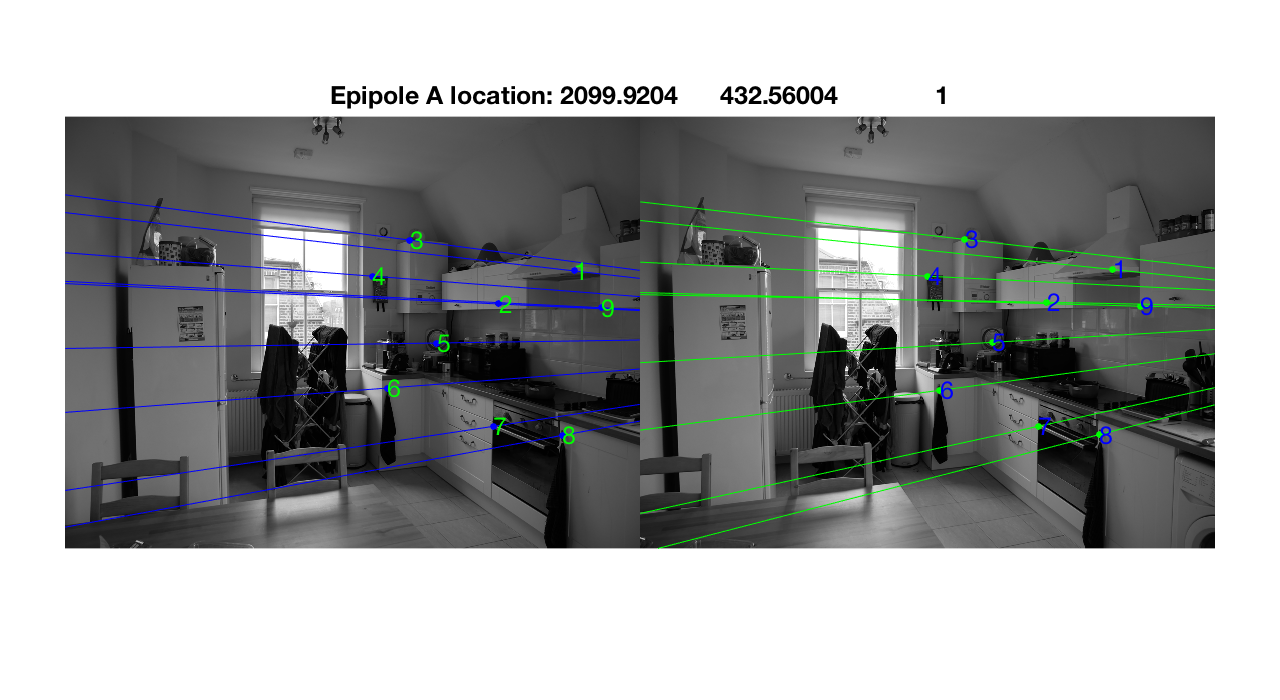
\includegraphics[width=\linewidth]{pic/q2_2_ab_A_0}
      \caption{Image A  vs. Image B.}
    \end{subfigure}
    ~
    \begin{subfigure}{0.45\linewidth}
        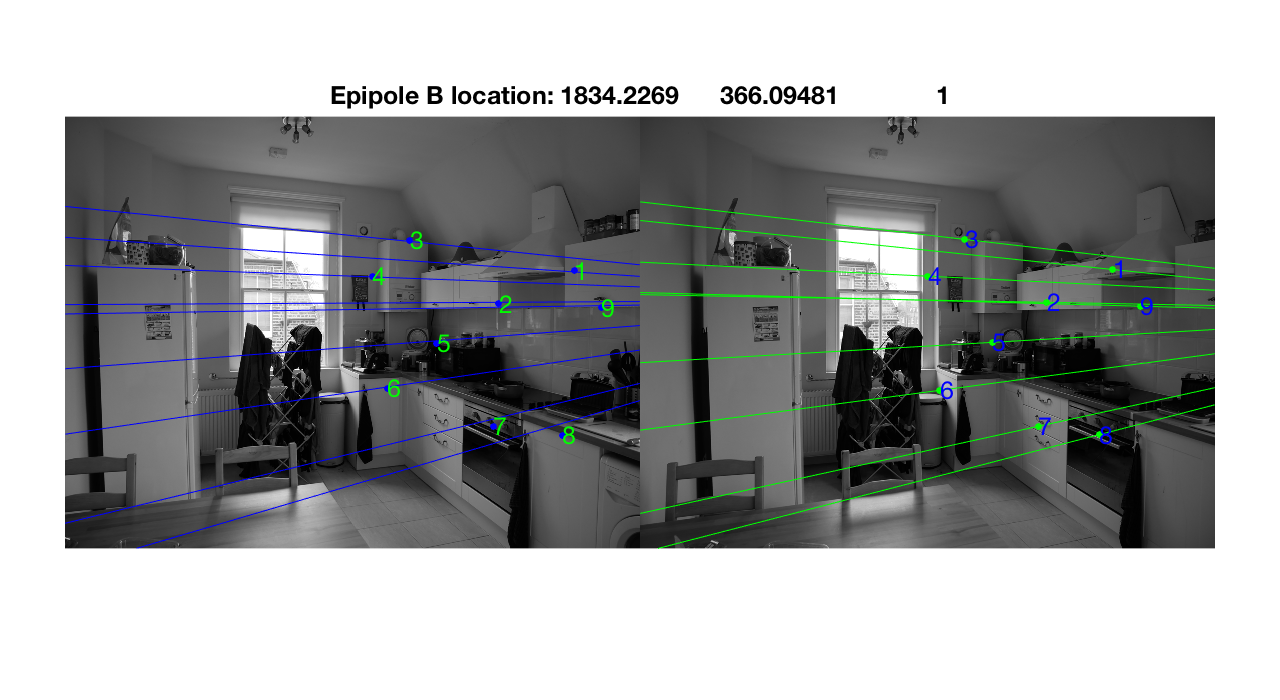
\includegraphics[width=\linewidth]{pic/q2_2_ab_B_0}
        \caption{Image B  vs. Image A.}
    \end{subfigure}

	\caption{Epipoles and epipolar lines.}
\end{figure}

\lstinputlisting[style=Matlab-editor]{src/q2_2_ab.m}
\newpage

\subsection*{Code for Q2.2.c and Q2.2.d with epipolar lines.}
\lstinputlisting[style=Matlab-editor]{src/q2_2_cd3.m}
\newpage

\subsection*{Code for Q2.2.c and Q2.2.d with horizontal lines.}

\begin{figure}[!ht]
  \captionsetup[subfigure]{position=b}
  \centering
    \begin{subfigure}{0.45\linewidth}
        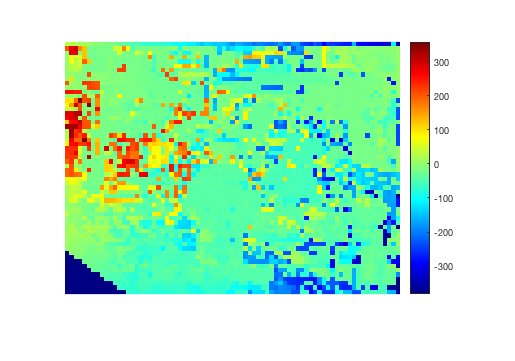
\includegraphics[width=\linewidth]{pic/q2_2_c1_dis}
      \caption{Disparity: Image 1  vs. Image 5, Epipolar Lines.}
    \end{subfigure}
    ~
    \begin{subfigure}{0.45\linewidth}
        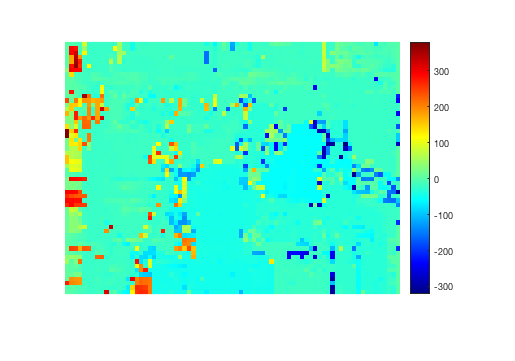
\includegraphics[width=\linewidth]{pic/q2_2_c2_dis}
        \caption{Disparity: Image 1  vs. Image 5, Horizontal Lines.}
    \end{subfigure}
    \\
    \begin{subfigure}{0.45\linewidth}
        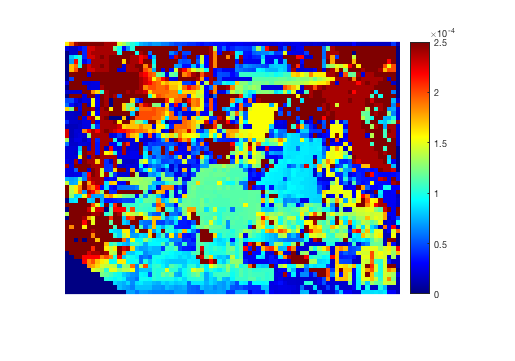
\includegraphics[width=\linewidth]{pic/q2_2_c1_depth}
      \caption{Depth: Image 1  vs. Image 5, Epipolar Lines.}
    \end{subfigure}
    ~
    \begin{subfigure}{0.45\linewidth}
        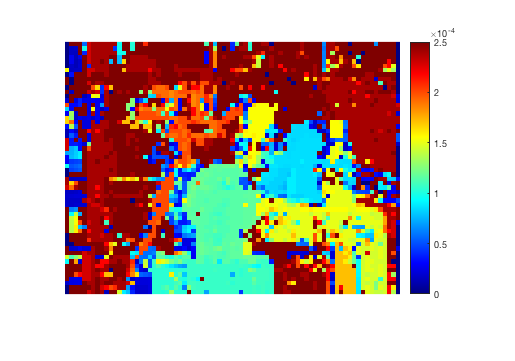
\includegraphics[width=\linewidth]{pic/q2_2_c2_depth}
        \caption{Depth: Image 1  vs. Image 5, Horizontal Lines.}
    \end{subfigure}

	\caption{Disparity and Depth.}
\end{figure}

\lstinputlisting[style=Matlab-editor]{src/q2_2_cd4.m}
\newpage


\end{document}
